% Options for packages loaded elsewhere
\PassOptionsToPackage{unicode}{hyperref}
\PassOptionsToPackage{hyphens}{url}
\documentclass[
  11pt,
]{article}
\usepackage{xcolor}
\usepackage{amsmath,amssymb}
\setcounter{secnumdepth}{-\maxdimen} % remove section numbering
\usepackage{iftex}
\ifPDFTeX
  \usepackage[T1]{fontenc}
  \usepackage[utf8]{inputenc}
  \usepackage{textcomp} % provide euro and other symbols
\else % if luatex or xetex
  \usepackage{unicode-math} % this also loads fontspec
  \defaultfontfeatures{Scale=MatchLowercase}
  \defaultfontfeatures[\rmfamily]{Ligatures=TeX,Scale=1}
\fi
\usepackage{lmodern}
\ifPDFTeX\else
  % xetex/luatex font selection
\fi
% Use upquote if available, for straight quotes in verbatim environments
\IfFileExists{upquote.sty}{\usepackage{upquote}}{}
\IfFileExists{microtype.sty}{% use microtype if available
  \usepackage[]{microtype}
  \UseMicrotypeSet[protrusion]{basicmath} % disable protrusion for tt fonts
}{}
\makeatletter
\@ifundefined{KOMAClassName}{% if non-KOMA class
  \IfFileExists{parskip.sty}{%
    \usepackage{parskip}
  }{% else
    \setlength{\parindent}{0pt}
    \setlength{\parskip}{6pt plus 2pt minus 1pt}}
}{% if KOMA class
  \KOMAoptions{parskip=half}}
\makeatother
\usepackage{longtable,booktabs,array}
\newcounter{none} % for unnumbered tables
\usepackage{calc} % for calculating minipage widths
% Correct order of tables after \paragraph or \subparagraph
\usepackage{etoolbox}
\makeatletter
\patchcmd\longtable{\par}{\if@noskipsec\mbox{}\fi\par}{}{}
\makeatother
% Allow footnotes in longtable head/foot
\IfFileExists{footnotehyper.sty}{\usepackage{footnotehyper}}{\usepackage{footnote}}
\makesavenoteenv{longtable}
\usepackage{graphicx}
\makeatletter
\newsavebox\pandoc@box
\newcommand*\pandocbounded[1]{% scales image to fit in text height/width
  \sbox\pandoc@box{#1}%
  \Gscale@div\@tempa{\textheight}{\dimexpr\ht\pandoc@box+\dp\pandoc@box\relax}%
  \Gscale@div\@tempb{\linewidth}{\wd\pandoc@box}%
  \ifdim\@tempb\p@<\@tempa\p@\let\@tempa\@tempb\fi% select the smaller of both
  \ifdim\@tempa\p@<\p@\scalebox{\@tempa}{\usebox\pandoc@box}%
  \else\usebox{\pandoc@box}%
  \fi%
}
% Set default figure placement to htbp
\def\fps@figure{htbp}
\makeatother
\setlength{\emergencystretch}{3em} % prevent overfull lines
\providecommand{\tightlist}{%
  \setlength{\itemsep}{0pt}\setlength{\parskip}{0pt}}
% ---------------------------------------------------------------------------
% Shared LaTeX style for Lab A - Electronics reports.
% Used by build_pdf.sh via `pandoc --include-in-header`.
% Engine: tectonic (XeTeX), so fontspec is available.
% ---------------------------------------------------------------------------

% --- Page geometry: A4 with the same comfortable margins as the vault export.
\usepackage[a4paper,top=18mm,bottom=20mm,left=16mm,right=16mm]{geometry}

% --- Times-like body font. Math is left in the default font, which matches how
%     the Obsidian (MathJax) export looks.
\usepackage{fontspec}
\setmainfont{texgyretermes}[
  Extension      = .otf,
  UprightFont    = *-regular,
  BoldFont       = *-bold,
  ItalicFont     = *-italic,
  BoldItalicFont = *-bolditalic,
]

% --- Colours.
\usepackage{xcolor}
\definecolor{figcap}{HTML}{0B5FB0}   % blue used for italic "*Figure N: ...*" captions (center-images.lua)
\definecolor{labteal}{HTML}{006b73}  % teal used for \figcap{...} in report YAML / markdown
\newcommand{\figcap}[1]{\begin{center}\textcolor{labteal}{\textit{#1}}\end{center}}

% --- Subsubsection headings indented 2em (matches Obsidian export / report YAML).
\makeatletter
\renewcommand{\subsubsection}{\@startsection{subsubsection}{3}{2em}{-3.25ex plus -1ex minus -.2ex}{1.5ex plus .2ex}{\normalfont\normalsize\bfseries}}
\makeatother

% --- Footer "-- N of M --", centered, on every page (matches the reference).
\usepackage{fancyhdr}
\usepackage{lastpage}
\newcommand{\labfooter}{\small -- \thepage\ of \pageref{LastPage} --}
\fancypagestyle{labreport}{%
  \fancyhf{}%
  \renewcommand{\headrulewidth}{0pt}%
  \fancyfoot[C]{\labfooter}%
}
\pagestyle{labreport}
% First page of an article uses the "plain" style; give it the same footer.
\fancypagestyle{plain}{%
  \fancyhf{}%
  \renewcommand{\headrulewidth}{0pt}%
  \fancyfoot[C]{\labfooter}%
}

% --- Keep headings, figures, and paragraphs together across page breaks.
\usepackage{needspace}
\usepackage{etoolbox}
\clubpenalty=10000
\widowpenalty=10000
\displaywidowpenalty=10000
\raggedbottom

% --- Keep bullet/numbered lists intact: do not break between a list and its
%     lead-in line, nor between individual items.
\makeatletter
\@beginparpenalty=9999
\@itempenalty=9999
\makeatother
\pretocmd{\section}{\Needspace{10\baselineskip}}{}{}
\pretocmd{\subsection}{\Needspace{10\baselineskip}}{}{}
\pretocmd{\subsubsection}{\Needspace{8\baselineskip}}{}{}
\pretocmd{\paragraph}{\Needspace{8\baselineskip}}{}{}
\pretocmd{\subparagraph}{\Needspace{6\baselineskip}}{}{}
\usepackage{bookmark}
\IfFileExists{xurl.sty}{\usepackage{xurl}}{} % add URL line breaks if available
\urlstyle{same}
\hypersetup{
  hidelinks,
  pdfcreator={LaTeX via pandoc}}

\author{}
\date{}

\begin{document}

\section{Lab 7: Operational Amplifiers --- Preliminary
Report}\label{lab-7-operational-amplifiers-preliminary-report}

\textbf{Students:} Shai Livshits · 208632216 ~\textbar~ Dan Masad ·
206505307 \textbf{Date:} June 26, 2026 \textbf{Course:} Lab A ---
Electronics, TAU Faculty of Engineering, Semester B 2025-2026

\begin{center}\rule{0.5\linewidth}{0.5pt}\end{center}

\newpage

\subsection{1. Op-Amp Properties Table (Datasheet
Summary)}\label{op-amp-properties-table-datasheet-summary}

{\def\LTcaptype{none} % do not increment counter
\begin{longtable}[]{@{}
  >{\raggedright\arraybackslash}p{(\linewidth - 6\tabcolsep) * \real{0.2105}}
  >{\centering\arraybackslash}p{(\linewidth - 6\tabcolsep) * \real{0.2632}}
  >{\centering\arraybackslash}p{(\linewidth - 6\tabcolsep) * \real{0.2632}}
  >{\centering\arraybackslash}p{(\linewidth - 6\tabcolsep) * \real{0.2632}}@{}}
\toprule\noalign{}
\begin{minipage}[b]{\linewidth}\raggedright
Parameter
\end{minipage} & \begin{minipage}[b]{\linewidth}\centering
TL071M
\end{minipage} & \begin{minipage}[b]{\linewidth}\centering
TL061M
\end{minipage} & \begin{minipage}[b]{\linewidth}\centering
LM741
\end{minipage} \\
\midrule\noalign{}
\endhead
\bottomrule\noalign{}
\endlastfoot
Input offset voltage \(V_{io}\) & 3 mV (typ) & 3 mV (typ) & 1 mV (typ),
6 mV (max) \\
Large-signal voltage gain \(A_{OL}\) & 200 V/mV (typ) & 200 V/mV (typ) &
200 V/mV (typ) \\
CMRR & 86 dB (typ) & 80 dB (typ) & 90 dB (typ) \\
Slew rate \(SR\) (unity-gain) & 13 V/μs & 3.5 V/μs & 0.5 V/μs \\
Unity-gain bandwidth \(f_t\) / GBW & 3 MHz & 1 MHz & 1 MHz \\
\end{longtable}
}

\newpage

\subsection{2. Explanation of Op-Amp
Properties}\label{explanation-of-op-amp-properties}

\subsubsection{2.1 Definition of Each
Property}\label{definition-of-each-property}

\begin{itemize}
\tightlist
\item
  \textbf{Input offset voltage \(V_{io}\):} The differential DC voltage
  that must be applied between the inputs to force \(V_{out}=0\); arises
  from transistor mismatches in the input stage.
\item
  \textbf{Large-signal voltage gain \(A_{OL}\):} Ratio of output to
  differential input voltage in open loop, measured at DC with a large
  (but unsaturated) output swing.
\item
  \textbf{CMRR:} Ratio of differential gain to common-mode gain;
  indicates the op-amp's ability to reject signals common to both
  inputs. A high CMRR means the output responds only to the differential
  signal.
\item
  \textbf{Slew rate \(SR\):} Maximum rate of change of the output
  voltage (\(\mathrm{d}V_{out}/\mathrm{d}t\big|_{\max}\)). Caused by a
  current-limited internal capacitor that must charge/discharge at a
  finite rate.
\item
  \textbf{Unity-gain bandwidth / GBW:} \(f_t\) is the frequency at which
  open-loop gain falls to 1 (0 dB). GBW is the product of closed-loop
  gain and 3 dB bandwidth; in a single-pole model,
  \(f_t = \mathrm{GBW}\).
\end{itemize}

\subsubsection{2.2 Differences in Bandwidth-Related
Specifications}\label{differences-in-bandwidth-related-specifications}

All three quantities (\(f_t\), GBW, \(f_{-3\mathrm{dB}}\)) describe
frequency limitations but represent different things:

\begin{itemize}
\tightlist
\item
  \(f_t\) (unity-gain bandwidth) is the frequency where \(|A_{OL}|=1\);
  it is an \textbf{open-loop} property.
\item
  GBW (gain-bandwidth product) is \(|A_{CL}| \times f_{-3\mathrm{dB}}\)
  for the \textbf{closed-loop} circuit; for a single-pole op-amp, GBW
  \(= f_t\).
\item
  \(f_{-3\mathrm{dB}}\) is the \textbf{closed-loop} bandwidth at a
  specific gain; it depends on the circuit.
\end{itemize}

The datasheets may label these differently (e.g.~TL071/TL061 quote
``unity-gain bandwidth'' directly; LM741 quotes a ``gain-bandwidth
product''). In the single-pole model they are identical, but multi-pole
op-amps can have \(f_t < \mathrm{GBW}\).

\newpage

\subsection{3. Voltage Definitions}\label{voltage-definitions}

We use our assigned numerical values
\(A = \dfrac{\mathrm{DEF}}{100} = \dfrac{307}{100} = 3.07\,\mathrm{V}\)
and \(B = 10\,\mathrm{V}\) (both positive), with
\(V(t) = A\sin(\omega t)\) unless noted.

\subsubsection{\texorpdfstring{3.1
\(V(t) = A\sin(\omega t)\)}{3.1 V(t) = A\textbackslash sin(\textbackslash omega t)}}\label{vt-asinomega-t}

{\def\LTcaptype{none} % do not increment counter
\begin{longtable}[]{@{}
  >{\raggedright\arraybackslash}p{(\linewidth - 4\tabcolsep) * \real{0.3077}}
  >{\raggedright\arraybackslash}p{(\linewidth - 4\tabcolsep) * \real{0.3077}}
  >{\centering\arraybackslash}p{(\linewidth - 4\tabcolsep) * \real{0.3846}}@{}}
\toprule\noalign{}
\begin{minipage}[b]{\linewidth}\raggedright
Quantity
\end{minipage} & \begin{minipage}[b]{\linewidth}\raggedright
Expression
\end{minipage} & \begin{minipage}[b]{\linewidth}\centering
Value (\(A=3.07\,\mathrm{V}\))
\end{minipage} \\
\midrule\noalign{}
\endhead
\bottomrule\noalign{}
\endlastfoot
\(V_\text{amplitude}\) & \(A\) & \(3.07\,\mathrm{V}\) \\
\(V_\text{max}\) & \(A\) & \(3.07\,\mathrm{V}\) \\
\(V_\text{mean}\) & \(0\) & \(0\,\mathrm{V}\) \\
\(V_{pp}\) & \(2A\) & \(6.14\,\mathrm{V}\) \\
\(V_\text{RMS}\) &
\(\dfrac{A}{\sqrt{2}}=\sqrt{\frac{1}{T}\int_0^T A^2\sin^2(\omega t)\,\mathrm{d}t}\)
& \(2.171\,\mathrm{V}\) \\
\end{longtable}
}

\subsubsection{\texorpdfstring{3.2 \(V(t) = A\sin(\omega t) + B\),
\(B > 0\)}{3.2 V(t) = A\textbackslash sin(\textbackslash omega t) + B, B \textgreater{} 0}}\label{vt-asinomega-t-b-b-0}

{\def\LTcaptype{none} % do not increment counter
\begin{longtable}[]{@{}
  >{\raggedright\arraybackslash}p{(\linewidth - 4\tabcolsep) * \real{0.3077}}
  >{\raggedright\arraybackslash}p{(\linewidth - 4\tabcolsep) * \real{0.3077}}
  >{\centering\arraybackslash}p{(\linewidth - 4\tabcolsep) * \real{0.3846}}@{}}
\toprule\noalign{}
\begin{minipage}[b]{\linewidth}\raggedright
Quantity
\end{minipage} & \begin{minipage}[b]{\linewidth}\raggedright
Expression
\end{minipage} & \begin{minipage}[b]{\linewidth}\centering
Value (\(A=3.07\,\mathrm{V}\), \(B=10\,\mathrm{V}\))
\end{minipage} \\
\midrule\noalign{}
\endhead
\bottomrule\noalign{}
\endlastfoot
\(V_\text{amplitude}\) & \(A\) & \(3.07\,\mathrm{V}\) \\
\(V_\text{max}\) & \(A + B\) & \(13.07\,\mathrm{V}\) \\
\(V_\text{mean}\) & \(B\) & \(10\,\mathrm{V}\) \\
\(V_{pp}\) & \(2A\) & \(6.14\,\mathrm{V}\) \\
\(V_\text{RMS}\) & \(\sqrt{\dfrac{A^2}{2} + B^2}\) &
\(10.233\,\mathrm{V}\) \\
\end{longtable}
}

\subsubsection{\texorpdfstring{3.3 \(V(t) = A\sin(\omega t) - B\),
\(B > 0\)}{3.3 V(t) = A\textbackslash sin(\textbackslash omega t) - B, B \textgreater{} 0}}\label{vt-asinomega-t---b-b-0}

{\def\LTcaptype{none} % do not increment counter
\begin{longtable}[]{@{}
  >{\raggedright\arraybackslash}p{(\linewidth - 4\tabcolsep) * \real{0.3077}}
  >{\raggedright\arraybackslash}p{(\linewidth - 4\tabcolsep) * \real{0.3077}}
  >{\centering\arraybackslash}p{(\linewidth - 4\tabcolsep) * \real{0.3846}}@{}}
\toprule\noalign{}
\begin{minipage}[b]{\linewidth}\raggedright
Quantity
\end{minipage} & \begin{minipage}[b]{\linewidth}\raggedright
Expression
\end{minipage} & \begin{minipage}[b]{\linewidth}\centering
Value (\(A=3.07\,\mathrm{V}\), \(B=10\,\mathrm{V}\))
\end{minipage} \\
\midrule\noalign{}
\endhead
\bottomrule\noalign{}
\endlastfoot
\(V_\text{amplitude}\) & \(A\) & \(3.07\,\mathrm{V}\) \\
\(V_\text{max}\) & \(A - B\) & \(-6.93\,\mathrm{V}\) \\
\(V_\text{mean}\) & \(-B\) & \(-10\,\mathrm{V}\) \\
\(V_{pp}\) & \(2A\) & \(6.14\,\mathrm{V}\) \\
\(V_\text{RMS}\) & \(\sqrt{\dfrac{A^2}{2} + B^2}\) &
\(10.233\,\mathrm{V}\) \\
\end{longtable}
}

Note: \(V_\text{RMS}\) is always non-negative (\(V_\text{RMS} \geq 0\))
even when \(V_\text{mean} < 0\), because it is the root of the
mean-square. The sign of \(V_\text{mean}\) does not affect
\(V_\text{RMS}\) --- both §3.2 and §3.3 give the same
\(V_\text{RMS}=10.233\,\mathrm{V}\).

\newpage

\subsection{4. Input Offset Voltage}\label{input-offset-voltage}

\subsubsection{\texorpdfstring{4.1 Non-Ideal Model of Figure 2 (Assume
\(V_{out} = 216\,\mathrm{mV}\))}{4.1 Non-Ideal Model of Figure 2 (Assume V\_\{out\} = 216\textbackslash,\textbackslash mathrm\{mV\})}}\label{non-ideal-model-of-figure-2-assume-v_out-216mathrmmv}

The input offset voltage \(V_{io}\) is the same quantity the datasheets
label \(V_{os}\) --- we use the course notation \(V_{io}\). If we assume
the op-amp is ideal in the offset sense (\(V_{io}=0\)), the output would
be \(V_{out}=0\); a real op-amp has \(V_{io}\neq 0\) and therefore a
non-zero output. The non-ideal op-amp is modelled by inserting a DC
source \(V_{io}\) in series with the non-inverting (\(+\)) input of an
otherwise ideal op-amp.

We are told to assume the (measured) output is
\(V_{out} = \mathrm{ABC}\,\mathrm{mV} = 216\,\mathrm{mV}\). In the
redrawn circuit, \(V_{io}\) sits in series with the \(+\) terminal and
is amplified by the non-inverting gain to produce the observed
\(V_{out}\).

\pandocbounded{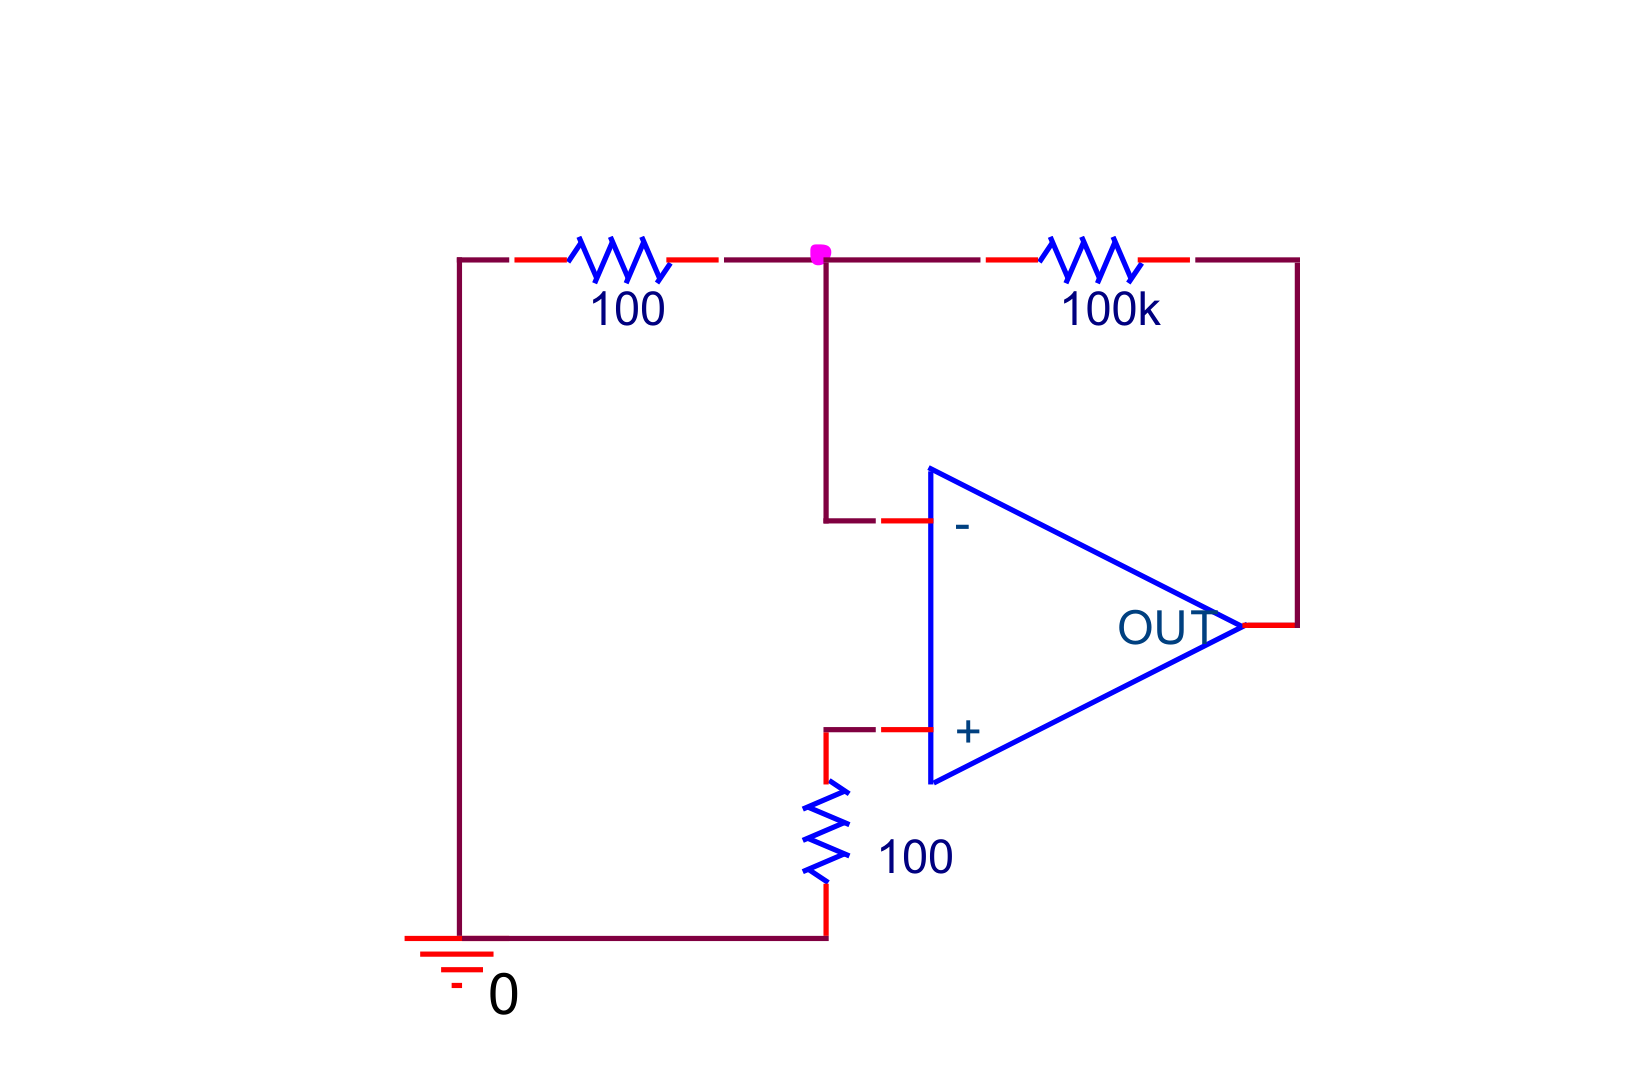
\includegraphics[keepaspectratio]{assets/figure2.png}}
\nopagebreak[4]

\begin{center}\textcolor{labteal}{\textit{Figure 1 - Figure 2: Inverting amplifier used to observe input offset voltage ($R_{in}=100\,\Omega$, $R_f=100\,\mathrm{k}\Omega$).}}\end{center}

\subsubsection{\texorpdfstring{4.2 Calculation of \(V_{io}\) and Its
Measurability}{4.2 Calculation of V\_\{io\} and Its Measurability}}\label{calculation-of-v_io-and-its-measurability}

With \(V_{in}=0\), the offset is amplified by the non-inverting gain
\(\left(1+R_f/R_{in}\right)\), so inverting the relation gives
\(V_{io}\) from the assumed output:

\[V_{out} = V_{io}\left(1 + \frac{R_f}{R_{in}}\right) \;\Rightarrow\; V_{io} = \frac{V_{out}}{1 + R_f/R_{in}}\]

\[V_{io} = \frac{216\,\mathrm{mV}}{1 + \dfrac{100\,\mathrm{k}\Omega}{100\,\Omega}} = \frac{216\,\mathrm{mV}}{1001} \approx 216\,\mu\mathrm{V}\]

This is in the \textbf{microvolt} range --- physically reasonable for a
real op-amp (datasheet \(V_{io}\) is typically 1--6 mV).

\textbf{Is it measurable?} Not directly:
\(V_{io}\approx 216\,\mu\mathrm{V}\) is far below the
\(\approx 50\,\mathrm{mV}\) lab noise floor, so it cannot be read at the
input terminals.

\textbf{How to find \(V_{io}\):} keep the circuit in its linear
operating region (output not saturated) and determine the closed-loop
gain \(G = 1 + R_f/R_{in}\). Then, for any output \(V_{out}\) measured
within the operating region, recover the offset as
\(V_{io} = V_{out}/G\).

\subsubsection{4.3 BJT Differential Pair --- Bias Point
Simulation}\label{bjt-differential-pair-bias-point-simulation}

Figure 3 shows the first-stage differential pair that emulates the
asymmetry causing offset:

\begin{itemize}
\tightlist
\item
  \(R_7 = 500 + \mathrm{ABC} = 500 + 216 = 716\,\Omega\)
\item
  \(R_8 = 500 + \mathrm{DEF} = 500 + 307 = 807\,\Omega\)
\item
  \(I_1 = 1\,\mathrm{mA}\), \(V_4 = 15\,\mathrm{V}\),
  \(R_4 = R_6 = 3\,\mathrm{k}\Omega\)
\end{itemize}

\pandocbounded{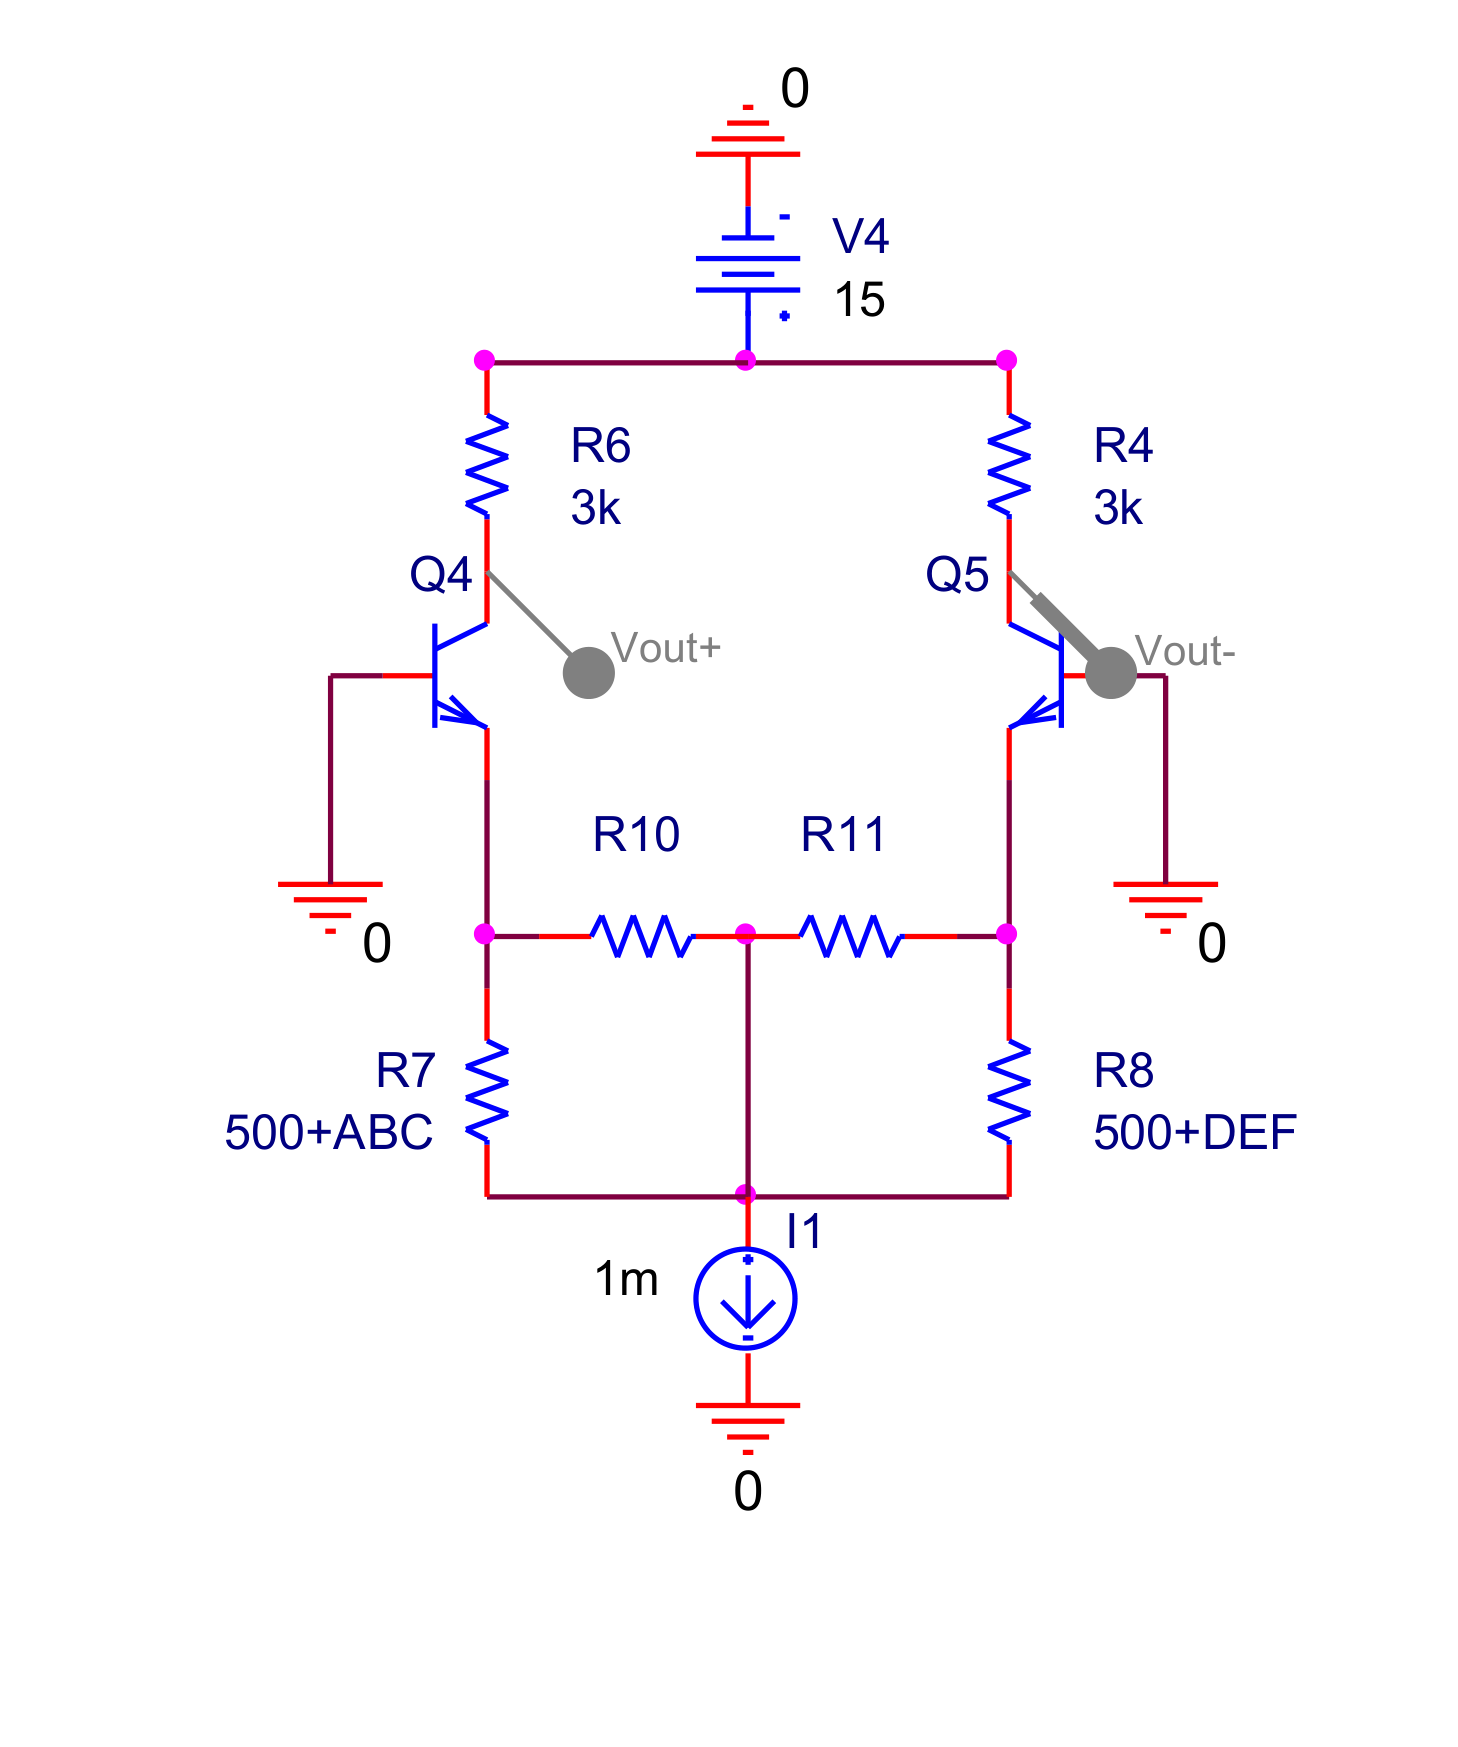
\includegraphics[keepaspectratio]{assets/figure3.png}}
\nopagebreak[4]

\begin{center}\textcolor{labteal}{\textit{Figure 2 - Figure 3: BJT differential pair with potentiometer $R_{10}$–$R_{11}$ for offset null.}}\end{center}

\textbf{Analytical estimate} (with \(R_{10}, R_{11}\) disconnected,
\(V_{BE}\) equal for both transistors):

\[\frac{I_{E4}}{I_{E5}} = \frac{R_8}{R_7} = \frac{807}{716} \approx 1.127\]

\[I_{E4} = \frac{R_8}{R_7+R_8}\times I_1 = \frac{807}{1523}\times 1\,\mathrm{mA} \approx 0.530\,\mathrm{mA}, \quad I_{E5} \approx 0.470\,\mathrm{mA}\]

\[V_{out+} = 15 - 0.530\times 3 = 13.41\,\mathrm{V}, \quad V_{out-} = 15 - 0.470\times 3 = 13.59\,\mathrm{V}\]

\begin{quote}
\textbf{{[}SIMULATION NEEDED --- 4.3{]}} Run a PSpice bias-point
simulation of Figure 3 with \(R_{10}, R_{11}\) disconnected. Record
\(V_{out+}\) and \(V_{out-}\) (no print required).
\end{quote}

\paragraph{4.3.1 Potentiometer Ratio for Zero
Output}\label{potentiometer-ratio-for-zero-output}

For equal collector currents (\(I_{C4} = I_{C5}\)), the effective
emitter resistance of each branch must be equal:

\[R_7 + R_{10} = R_8 + R_{11}\]
\[R_{10} - R_{11} = R_8 - R_7 = 807 - 716 = 91\,\Omega\]

For a 10 kΩ potentiometer (\(R_{10}+R_{11}=10\,\mathrm{k}\Omega\)):

\[R_{10} = \frac{10000 + 91}{2} = 5045.5\,\Omega, \quad R_{11} = 4954.5\,\Omega\]
\[\frac{R_{10}}{R_{10}+R_{11}} \approx 0.505 \quad (50.5\%)\]

\paragraph{4.3.2 Simulation with Chosen
Ratio}\label{simulation-with-chosen-ratio}

\begin{quote}
\textbf{{[}SIMULATION NEEDED --- 4.3.2{]}} Simulate Figure 3 with
\(R_{10}=5045.5\,\Omega\), \(R_{11}=4954.5\,\Omega\). Confirm
\(V_{out+}\approx V_{out-}\) (no print required).
\end{quote}

\paragraph{4.3.3 10\% Change in Potentiometer
Ratio}\label{change-in-potentiometer-ratio}

If the ratio changes by 10\% from the balanced point,
e.g.~\(R_{10}/R_{pot} = 0.505 \times 1.1 = 0.556\), a small asymmetry
reappears.

\begin{quote}
\textbf{{[}SIMULATION NEEDED --- 4.3.3{]}} Simulate with the ±10\% ratio
perturbation and attach a print. Record
\(\Delta V = V_{out+} - V_{out-}\).
\end{quote}

\newpage

\subsection{5. CMRR}\label{cmrr}

\subsubsection{\texorpdfstring{5.1 Definition of CMRR and Differential
Gain
\(A_d\)}{5.1 Definition of CMRR and Differential Gain A\_d}}\label{definition-of-cmrr-and-differential-gain-a_d}

\[\mathrm{CMRR} = \left|\frac{A_d}{A_{cm}}\right| \quad \text{(dimensionless)}, \qquad \mathrm{CMRR_{dB}} = 20\log_{10}\!\left|\frac{A_d}{A_{cm}}\right| \quad \text{(dB)}\]

where \(A_d = V_{out}/V_{diff}\) is the differential gain and
\(A_{cm} = V_{out}/V_{cm}\) is the common-mode gain.

Given \(\mathrm{CMRR} = 60 + \mathrm{AB} = 60 + 21 = 81\,\mathrm{dB}\)
and \(A_{cm} = \dfrac{\mathrm{DEF}}{1000} = \dfrac{307}{1000} = 0.307\):

\[A_d = A_{cm}\times 10^{\mathrm{CMRR_{dB}}/20} = 0.307\times 10^{81/20} = 0.307\times 10^{4.05} \approx 0.307\times 11{,}220 \approx 3.44\times 10^{3}\]

\subsubsection{\texorpdfstring{5.2 Transfer Functions \(A_4\) and
\(A_5\) (\(=V_{out}/V_{in}\)) for Figures 4 and
5}{5.2 Transfer Functions A\_4 and A\_5 (=V\_\{out\}/V\_\{in\}) for Figures 4 and 5}}\label{transfer-functions-a_4-and-a_5-v_outv_in-for-figures-4-and-5}

\pandocbounded{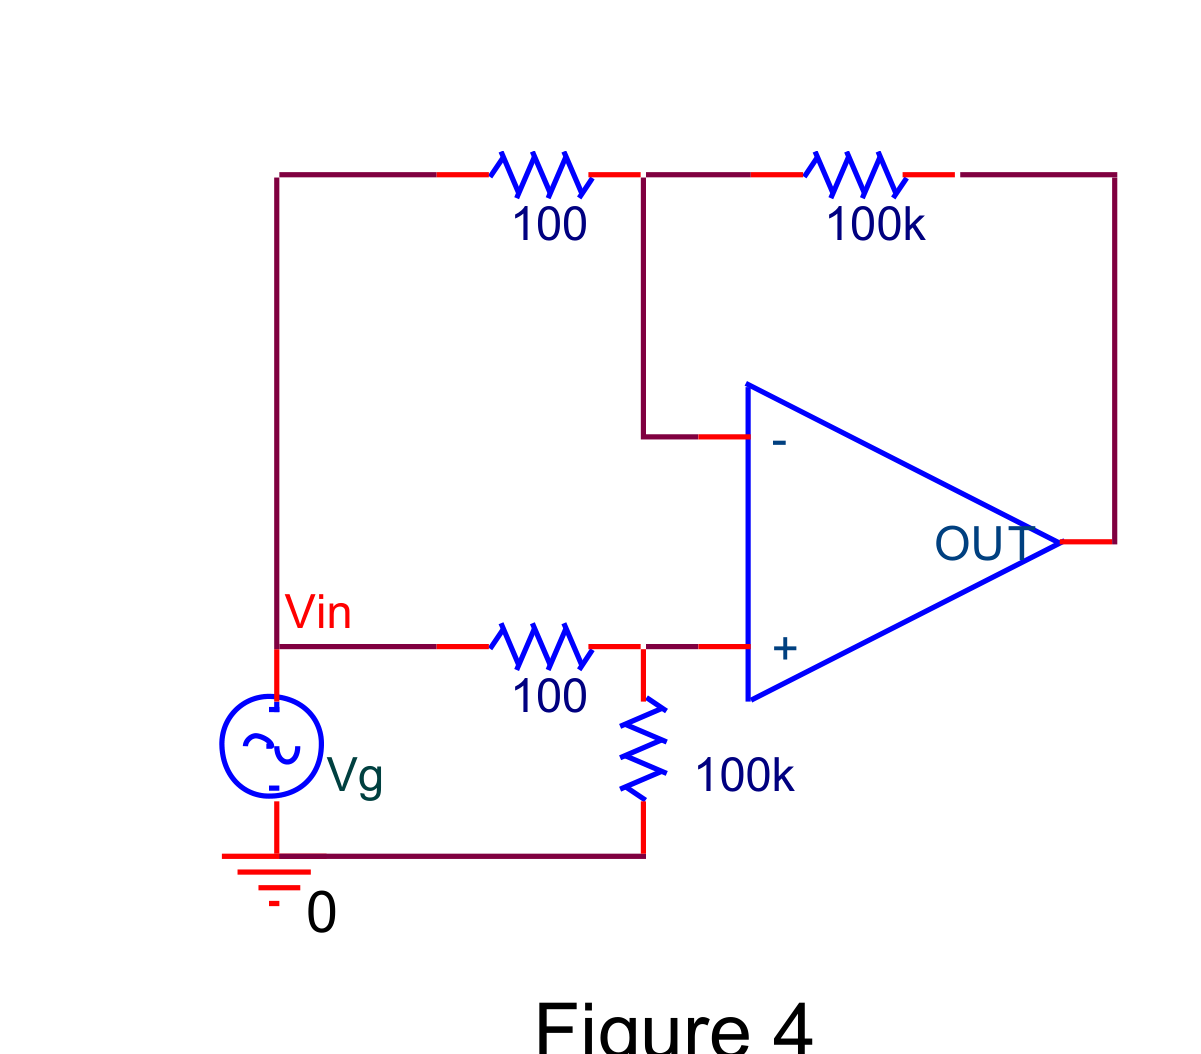
\includegraphics[keepaspectratio]{assets/figure4.png}}
\nopagebreak[4]

\begin{center}\textcolor{labteal}{\textit{Figure 3 - Figure 4: Common-mode circuit for measuring $A_{cm}$ (ideal output $V_{out}=0$).}}\end{center}

\pandocbounded{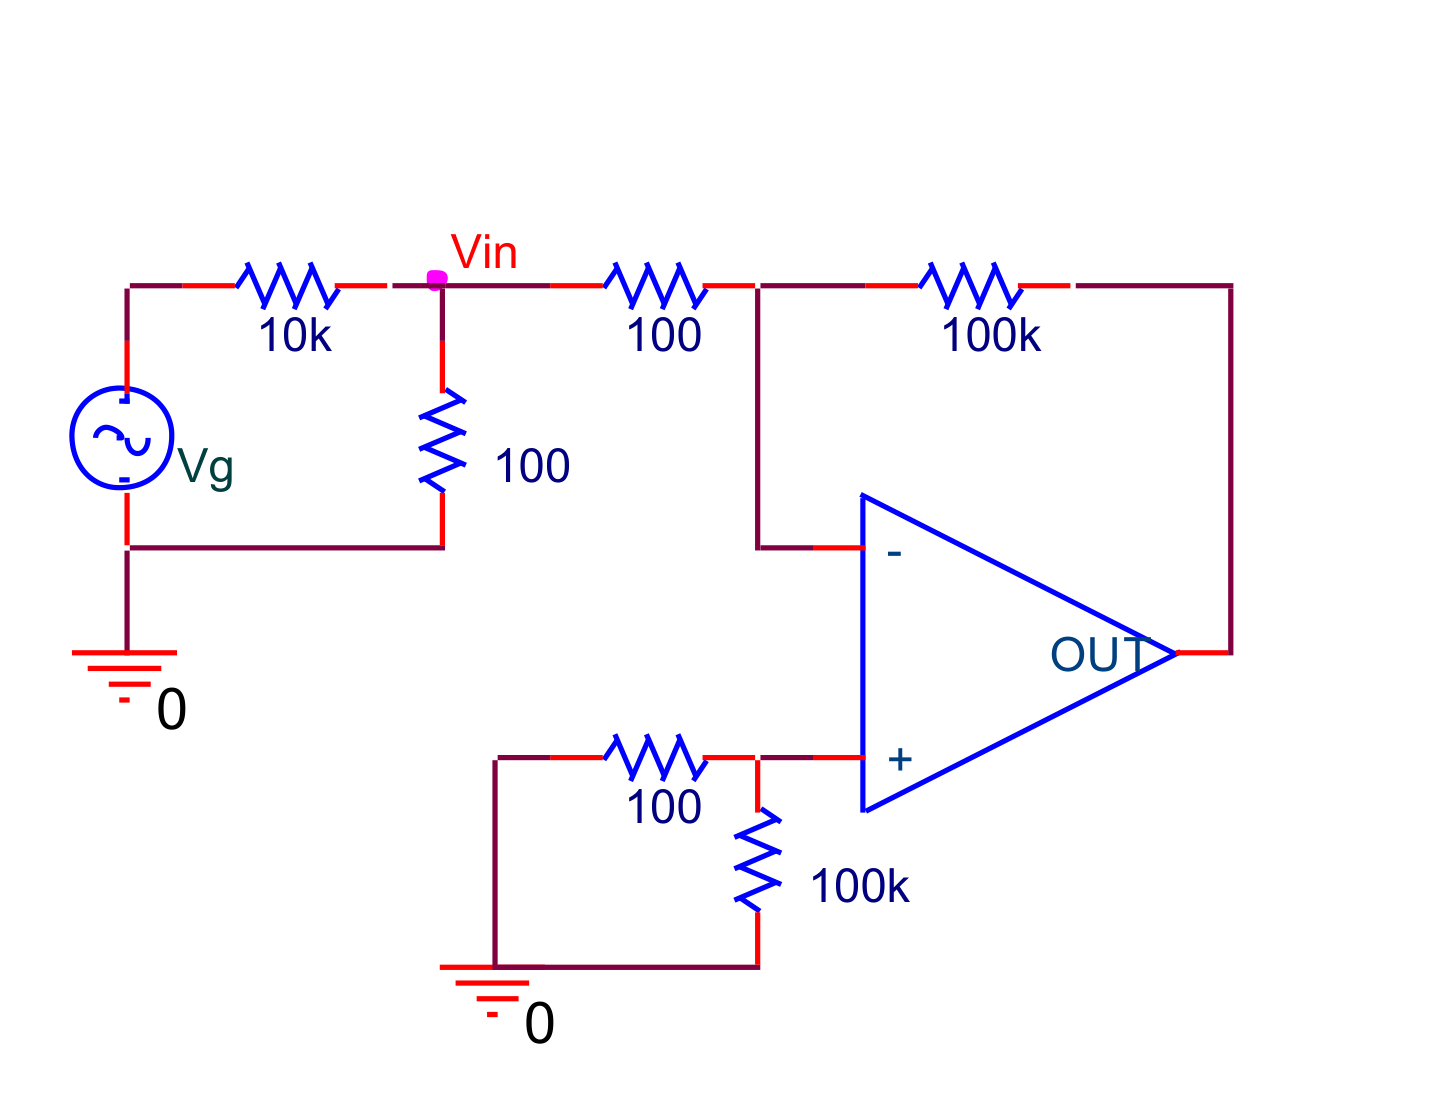
\includegraphics[keepaspectratio]{assets/figure5.png}}
\nopagebreak[4]

\begin{center}\textcolor{labteal}{\textit{Figure 4 - Figure 5: Differential (inverting) amplifier for measuring $A_d$ ($A_5=-R_f/R_{in}=-1000$).}}\end{center}

\textbf{Figure 4} (common-mode circuit): both inputs are driven by the
same common-mode input \(V_{in}\). For an ideal op-amp with matched
resistors, the common-mode signal is rejected, so

\[V_{-}=V_{in}\frac{1000}{1001}\rightarrow V_{out}=0 \] thus:
\[A_4 = \frac{V_{out}}{V_{in}} = 0 \quad \]

A real op-amp produces a small nonzero output, so this circuit is used
to measure the common-mode gain \(A_{cm}\).

\textbf{Figure 5} (differential / inverting amplifier): with the signal
applied differentially,

\[A_5 = \frac{V_{out}}{V_{in}} = -\frac{R_f}{R_{in}} = -\frac{100\,\mathrm{k}\Omega}{100\,\Omega} = -1000\]

This circuit measures the differential gain \(A_d\).

\textbf{Circuit assignment and CMRR expression:} Figure 5 (differential,
\(A_5=-1000\)) measures \(A_d\); Figure 4 (common-mode, ideal
\(V_{out}=0\)) measures \(A_{cm}\). Hence \(A_d = A_5\) and
\(A_{cm} = A_4\) (the small, real common-mode gain), and

\[\mathrm{CMRR} = \left|\frac{A_d}{A_{cm}}\right| = \left|\frac{A_5}{A_4}\right|\]

\subsubsection{5.3}\label{section}

Because the ideal common-mode output is zero, the real common-mode
output \(A_{cm}V_{in}\) is tiny; a large input is needed to lift it
above the noise floor, so the 2--4 VRMS range (rather than 50 m--300
mVRMS) is the correct choice.

\subsubsection{5.4}\label{section-1}

Without the series input resistors the closed-loop gain would be
determined by the op-amp's own (uncontrolled) input impedance rather
than a known resistor ratio. The resistors define the gain precisely;
without them the measurement of \(A_d\) or \(A_{cm}\) would be
unreliable. Additionally, mismatched resistors are the dominant source
of finite CMRR in a real difference amplifier; specifying exact values
is essential for a quantitative CMRR measurement.

Alongside the resistor choice, the input amplitude must also be set
appropriately for the differential measurement: for the differential
amplification (Figure 5, \(|A_5| = R_f/R_{in} = 1000\)) we use an input
amplitude of \textbf{50 m--300 mVRMS} (see §5.3). This keeps the
amplified output \(V_{out} = A_5 V_{in}\) within the
\(\pm 15\,\mathrm{V}\) supply rails and the op-amp in its linear region,
so that the gain --- and hence the extracted CMRR --- is measured
accurately rather than from a clipped (distorted) waveform.

\newpage

\subsection{6. Slew-Rate and Full-Power
Bandwidth}\label{slew-rate-and-full-power-bandwidth}

\subsubsection{6.1 Formulas and
Definitions}\label{formulas-and-definitions}

\[\mathrm{SR} = \left.\frac{\mathrm{d}V_{out}}{\mathrm{d}t}\right|_{\max} \quad [\mathrm{V/\mu s}]\]

\[\mathrm{FPBW} = \frac{\mathrm{SR}}{2\pi\, V_{om}} \quad [\mathrm{Hz}]\]

where \(V_{om}\) is the maximum undistorted output amplitude (typically
\(V_{CC}-2\,\mathrm{V}\)).

\textbf{Relationship:} FPBW is the highest frequency at which the op-amp
can produce a full-swing sinusoidal output (\(V_{om}\)) without SR
distortion. A sine wave requires
\(\mathrm{d}V_{out}/\mathrm{d}t|_{\max} = 2\pi f V_{om} \leq \mathrm{SR}\);
at \(f = \mathrm{FPBW}\) this limit is exactly reached.

\subsubsection{6.2 SR vs.~Finite
Bandwidth}\label{sr-vs.-finite-bandwidth}

{\def\LTcaptype{none} % do not increment counter
\begin{longtable}[]{@{}
  >{\raggedright\arraybackslash}p{(\linewidth - 4\tabcolsep) * \real{0.3333}}
  >{\raggedright\arraybackslash}p{(\linewidth - 4\tabcolsep) * \real{0.3333}}
  >{\raggedright\arraybackslash}p{(\linewidth - 4\tabcolsep) * \real{0.3333}}@{}}
\toprule\noalign{}
\begin{minipage}[b]{\linewidth}\raggedright
\end{minipage} & \begin{minipage}[b]{\linewidth}\raggedright
Slew-rate limiting
\end{minipage} & \begin{minipage}[b]{\linewidth}\raggedright
Finite (closed-loop) bandwidth
\end{minipage} \\
\midrule\noalign{}
\endhead
\bottomrule\noalign{}
\endlastfoot
\textbf{Effect on output} & Output ramp at constant slope \(\pm\)SR;
triangular rather than sinusoidal & Output sinusoidal but attenuated at
\(f > f_{-3\mathrm{dB}}\) \\
\textbf{Depends on} & Signal amplitude and frequency & Signal frequency
only (not amplitude) \\
\textbf{Electronic origin} & A compensation capacitor inside the op-amp
can only charge/discharge at a finite current (\(I_{bias}\));
\(\mathrm{SR}=I_{bias}/C\) & The single dominant pole formed by the
compensation capacitor limits high-frequency open-loop gain, reducing
closed-loop BW \\
\end{longtable}
}

SR is a \textbf{large-signal} (nonlinear) phenomenon; finite BW is a
\textbf{small-signal} (linear) limitation.

\subsubsection{6.3 Maximum Input Amplitude Before SR Limiting (Figure
6)}\label{maximum-input-amplitude-before-sr-limiting-figure-6}

\pandocbounded{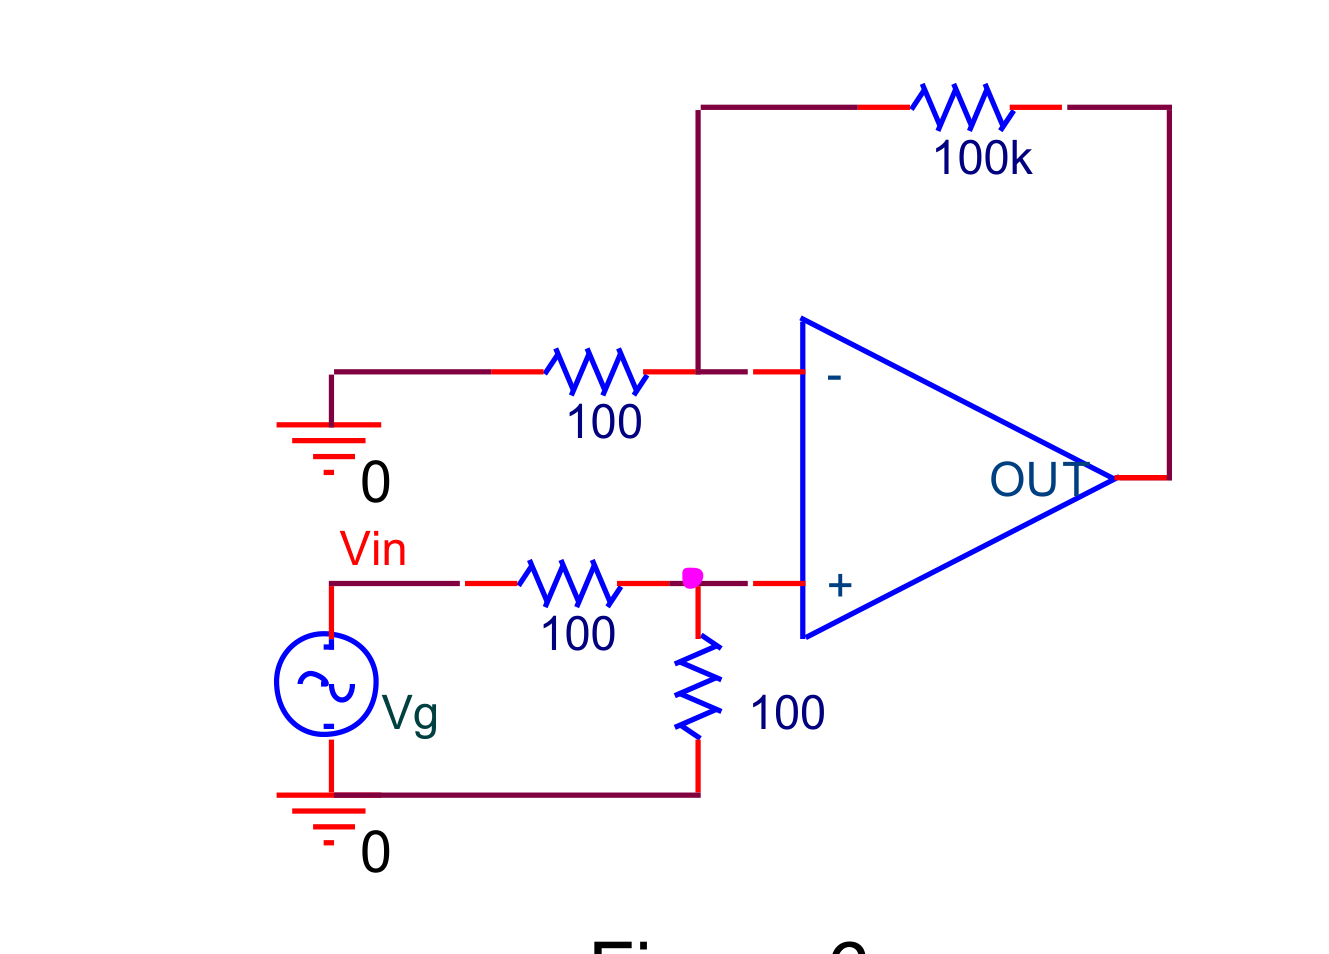
\includegraphics[keepaspectratio]{assets/figure6.png}}
\nopagebreak[4]

\begin{center}\textcolor{labteal}{\textit{Figure 5 - Figure 6: Circuit used for slew-rate measurement ($R_{in}=100\,\Omega$, $R_f=100\,\mathrm{k}\Omega$, $|A_v|=1000$).}}\end{center}

For a sinusoidal input at frequency \(f\), the output slope requirement
is:

\[\left.\frac{\mathrm{d}V_{out}}{\mathrm{d}t}\right|_{\max} = 2\pi f\,|A_v|\,V_{in,pk}\]

Setting this equal to SR (SR-limit onset):

\[V_{in,pk}^{\max} = \frac{\mathrm{SR}}{2\pi f\,|A_v|}\]

For the LM741 simulation (\(\mathrm{SR}=0.5\,\mathrm{V/\mu s}\),
\(|A_v|=1000\), \(f=1\,\mathrm{kHz}\)):

\[V_{in,pk}^{\max} = \frac{0.5\times10^6}{2\pi\times10^3\times10^3} \approx 80\,\mathrm{mV_{pk}} \approx 56\,\mathrm{mVRMS}\]

\subsubsection{6.4 Full-Power Bandwidth for Two Supply
Voltages}\label{full-power-bandwidth-for-two-supply-voltages}

\[\mathrm{FPBW} = \frac{\mathrm{SR}}{2\pi\,V_{om}}\]

For LM741, \(\mathrm{SR}=0.5\,\mathrm{V/\mu s}\),
\(V_{om}\approx V_{CC}-2\,\mathrm{V}\):

{\def\LTcaptype{none} % do not increment counter
\begin{longtable}[]{@{}
  >{\centering\arraybackslash}p{(\linewidth - 4\tabcolsep) * \real{0.3333}}
  >{\centering\arraybackslash}p{(\linewidth - 4\tabcolsep) * \real{0.3333}}
  >{\centering\arraybackslash}p{(\linewidth - 4\tabcolsep) * \real{0.3333}}@{}}
\toprule\noalign{}
\begin{minipage}[b]{\linewidth}\centering
Supply \(V_{CC}\)
\end{minipage} & \begin{minipage}[b]{\linewidth}\centering
\(V_{om}\)
\end{minipage} & \begin{minipage}[b]{\linewidth}\centering
FPBW
\end{minipage} \\
\midrule\noalign{}
\endhead
\bottomrule\noalign{}
\endlastfoot
\(\pm 15\,\mathrm{V}\) & \(13\,\mathrm{V}\) &
\(\dfrac{0.5\times10^6}{2\pi\times13}\approx 6.1\,\mathrm{kHz}\) \\
\(\pm 12\,\mathrm{V}\) & \(10\,\mathrm{V}\) &
\(\dfrac{0.5\times10^6}{2\pi\times10}\approx 8.0\,\mathrm{kHz}\) \\
\end{longtable}
}

These values are qualitative (actual op-amp unknown); they may not be
achievable in the lab, but are theoretically consistent with LM741
specifications.

\subsubsection{6.5 Output for Step-Function Input with Load
Capacitor}\label{output-for-step-function-input-with-load-capacitor}

With a capacitor \(C_L\) at the output and an ideal step
\(V_{in} = V_0\,u(t)\), the output \(V_{out}(t)\):

\textbf{Not SR-limited} (small \(V_0\), \$\textbar A\_v\textbar V\_0
\textless{} \$ SR threshold): The output rises exponentially with time
constant \(\tau = R_{out}C_L\) (or the closed-loop time constant
\(1/(2\pi f_{-3\mathrm{dB}})\)), approaching the final value
\(A_v\,V_0\).

\textbf{SR-limited} (large \(V_0\)): The output rises as a
\textbf{linear ramp} with slope SR until it reaches the final value
\(A_v V_0\), then settles. The larger \(V_0\), the longer the ramp
phase.

Qualitative sketch: - Non-SR-limited: smooth exponential approach to
\(A_v V_0\). - SR-limited: straight ramp at slope SR, then exponential
settling at the top.

\subsubsection{6.6 Scope Scale for SR
Observation}\label{scope-scale-for-sr-observation}

The LM741 SR \(\approx 0.5\,\mathrm{V/\mu s}\). A 10--15 V output swing
(full-scale) takes:

\[t_{slew} = \frac{\Delta V}{\mathrm{SR}} = \frac{15}{0.5} = 30\,\mu\mathrm{s}\]

To see this comfortably in 10 cm (10 divisions) across the screen:

\[\text{Scale} = \frac{30\,\mu\mathrm{s}}{3\text{ div}} \approx 10\,\mu\mathrm{s/div}\]

Recommended: \textbf{10 μs/div}, allowing the rising edge to span 3--4
divisions.

\subsubsection{6.7 Measuring SR in the
Lab}\label{measuring-sr-in-the-lab}

\begin{enumerate}
\def\labelenumi{\arabic{enumi}.}
\tightlist
\item
  Build Figure 6 with the appropriate gain.
\item
  Apply a \textbf{square wave} input at low frequency (e.g., 100 Hz),
  amplitude small enough that the output is SR-limited on the edges
  (check: output ramps linearly, not exponentially).
\item
  Set horizontal scale to \textasciitilde10 μs/div so the rising/falling
  edges span several divisions.
\item
  Use the cursors to measure \(\Delta V\) (vertical) and \(\Delta t\)
  (horizontal) on the linear portion of the rising edge.
\item
  \(\mathrm{SR} = \Delta V / \Delta t\).
\end{enumerate}

Do \textbf{not} use frequency sweeping to measure SR --- at higher
frequencies, additional distortion mechanisms unrelated to SR appear and
corrupt the measurement.

\newpage

\subsection{7. Gain-Bandwidth Product}\label{gain-bandwidth-product}

\subsubsection{7.1 Single-Pole Transfer Function and Bode
Plot}\label{single-pole-transfer-function-and-bode-plot}

\[A(j\omega) = \frac{A_0}{1 + j\omega/\omega_p} \quad\Rightarrow\quad |A(f)| = \frac{A_0}{\sqrt{1+(f/f_p)^2}}\]

Qualitative semi-log Bode magnitude:

\begin{itemize}
\tightlist
\item
  Flat at \(A_0\) (in dB) for \(f \ll f_p\)
\item
  Decreases at \(-20\,\mathrm{dB/decade}\) for \(f \gg f_p\)
\item
  Crosses 0 dB at \(f_t = A_0 f_p\) (unity-gain frequency)
\end{itemize}

\subsubsection{7.2 Unity-Gain BW Equals GBW in Single-Pole
Model}\label{unity-gain-bw-equals-gbw-in-single-pole-model}

For a single-pole model, \(f_t \approx A_0 f_p\) (since
\(f_t \gg f_p\)). The GBW product of the first pole is defined as
\(A_0\times f_p\). Thus:

\[f_t = A_0 f_p = \mathrm{GBW}\]

For a \textbf{multi-pole} op-amp, the gain falls faster above the first
pole (the second pole adds additional phase and gain roll-off), so
\(f_t < A_0 f_p\). Hence equality holds \textbf{if and only if} the
single-pole approximation is valid.

\subsubsection{\texorpdfstring{7.3 Numerical Example: \(A_0 = 10^5\),
\(f_p = 10\,\mathrm{Hz}\)}{7.3 Numerical Example: A\_0 = 10\^{}5, f\_p = 10\textbackslash,\textbackslash mathrm\{Hz\}}}\label{numerical-example-a_0-105-f_p-10mathrmhz}

\begin{itemize}
\tightlist
\item
  \textbf{Bode slope:} \(-20\,\mathrm{dB/decade}\) above
  \(f_p = 10\,\mathrm{Hz}\)
\item
  \textbf{Open-loop bandwidth} (−3 dB): \(f_p = 10\,\mathrm{Hz}\)
\item
  \textbf{Unity-gain bandwidth:}
  \(f_t = A_0 f_p = 10^5\times 10 = 1\,\mathrm{MHz}\)
\item
  \textbf{GBW} \(= f_t = 1\,\mathrm{MHz}\)
\end{itemize}

\subsubsection{\texorpdfstring{7.4 Gain at \(f = 10\,\mathrm{kHz}\) and
Frequency for
\(|A| = 10\)}{7.4 Gain at f = 10\textbackslash,\textbackslash mathrm\{kHz\} and Frequency for \textbar A\textbar{} = 10}}\label{gain-at-f-10mathrmkhz-and-frequency-for-a-10}

At \(f \gg f_p\): \(|A(f)| \approx A_0 f_p/f\)

\[|A(10\,\mathrm{kHz})| \approx \frac{10^5\times 10}{10^4} = 100 \quad(40\,\mathrm{dB})\]

\[|A(f)| = 10 \;\Rightarrow\; f = \frac{A_0 f_p}{10} = \frac{10^5\times 10}{10} = 100\,\mathrm{kHz}\]

\subsubsection{7.5 Closed-Loop Transfer Functions (Figures 7 and
8)}\label{closed-loop-transfer-functions-figures-7-and-8}

\pandocbounded{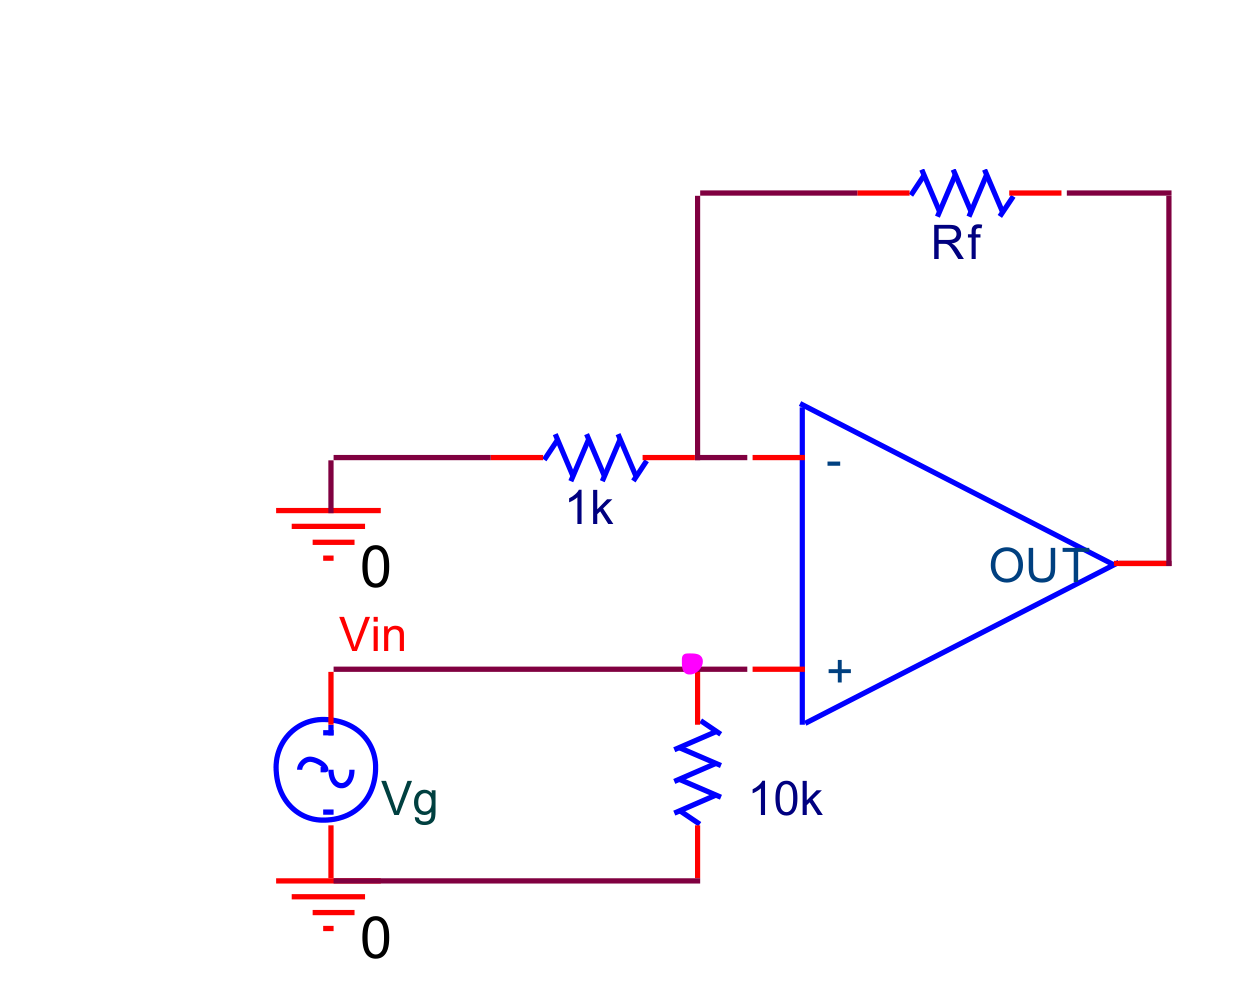
\includegraphics[keepaspectratio]{assets/figure7.png}}
\nopagebreak[4]

\begin{center}\textcolor{labteal}{\textit{Figure 6 - Figure 7: Non-inverting amplifier for GBW measurement ($R_1=1\,\mathrm{k}\Omega$ from the $-$ input to ground, $R_f$ variable, $10\,\mathrm{k}\Omega$ in series with the $+$ input).}}\end{center}

\pandocbounded{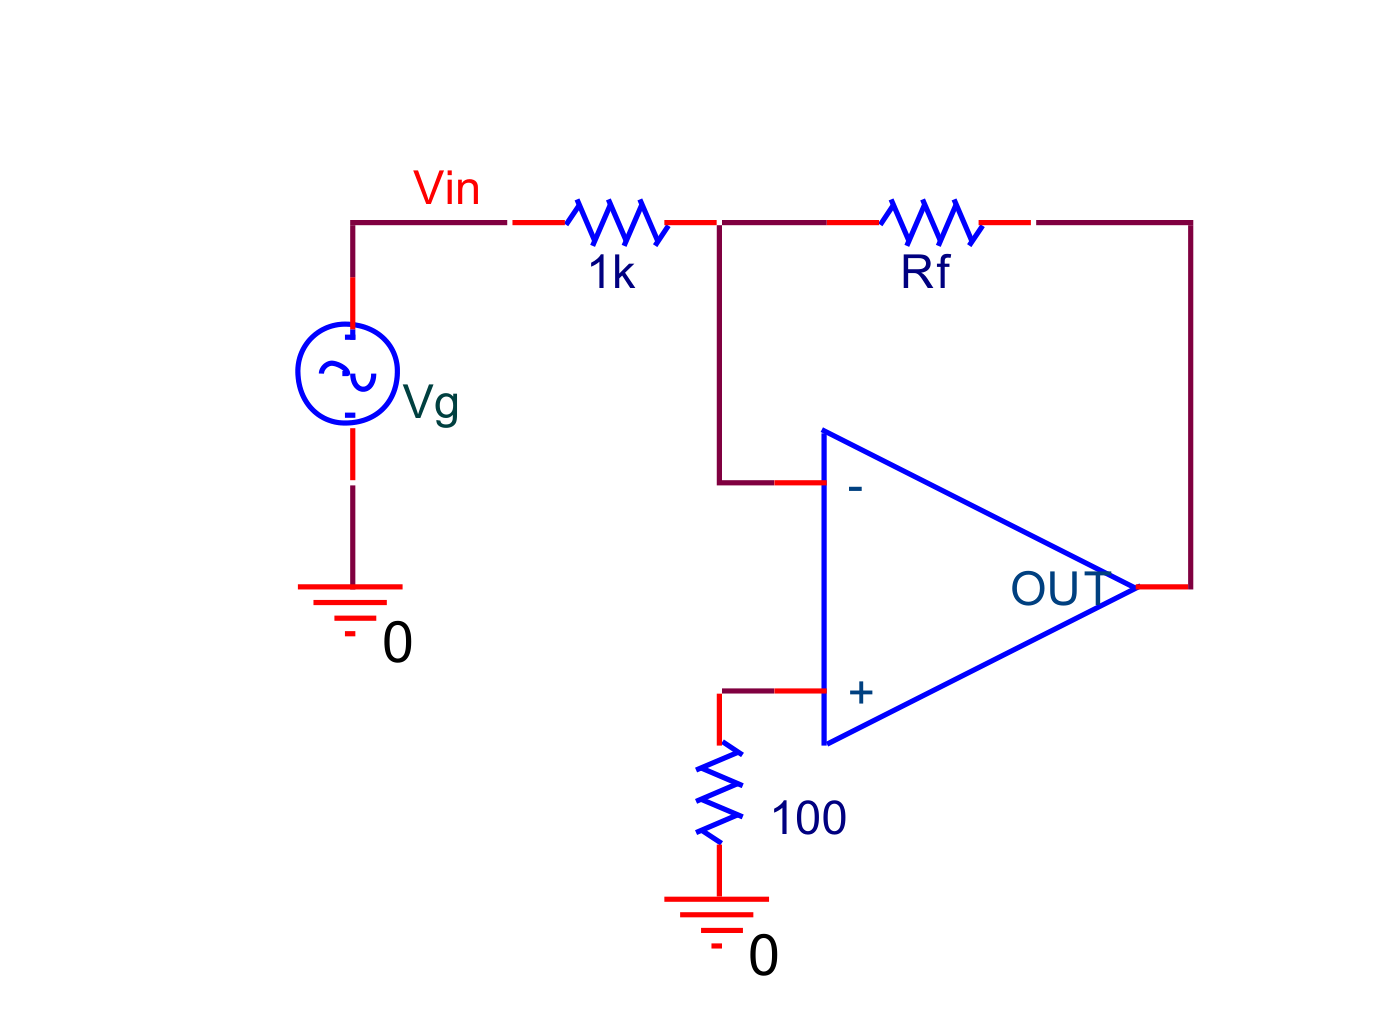
\includegraphics[keepaspectratio]{assets/figure8.png}}
\nopagebreak[4]

\begin{center}\textcolor{labteal}{\textit{Figure 7 - Figure 8: Inverting amplifier for GBW measurement ($R_1=1\,\mathrm{k}\Omega$, $R_f$ variable, $100\,\Omega$ from the $+$ input to ground).}}\end{center}

For a single-pole open-loop gain \(A(s) = A_0\omega_p/(s+\omega_p)\),
the closed-loop TFs are:

\textbf{Figure 7} (non-inverting --- the source drives the \(+\) input
through the \(10\,\mathrm{k}\Omega\) series resistor, \(R_1\) from \(-\)
to ground, \(R_f\) variable):

\[H_7(j\omega) = \left(1+\frac{R_f}{R_1}\right)\cdot\frac{1}{1+j\omega/\omega_{3\mathrm{dB}}}, \quad \omega_{3\mathrm{dB}} = \frac{\omega_t}{1+R_f/R_1}\]

\textbf{Figure 8} (inverting --- the source drives the \(-\) input
through \(R_1\), the \(+\) input is grounded through \(100\,\Omega\),
\(R_f\) variable):

\[H_8(j\omega) = -\frac{R_f}{R_1}\cdot\frac{1}{1+j\omega/\omega_{3\mathrm{dB}}}, \quad \omega_{3\mathrm{dB}} = \frac{\omega_t}{1+R_f/R_1}\]

Both share the same \(\omega_{3\mathrm{dB}}\) expression with
\(\omega_t = 2\pi f_t = 2\pi\,\mathrm{GBW}\). The closed-loop
\(-3\,\mathrm{dB}\) bandwidth is fixed by the \textbf{noise gain}
\(\left(1+R_f/R_1\right)\), which is identical for both topologies; only
the DC closed-loop gain magnitude differs (\(1+R_f/R_1\) for the
non-inverting circuit, \(R_f/R_1\) for the inverting one).

\subsubsection{7.6 GBW Product and Condition for
Equality}\label{gbw-product-and-condition-for-equality}

\[\mathrm{GBW}_7 = \left(1+\frac{R_f}{R_1}\right)\cdot\frac{f_t}{1+R_f/R_1} = f_t \qquad\text{(non-inverting)}\]

\[\mathrm{GBW}_8 = \frac{R_f}{R_1}\cdot\frac{f_t}{1+R_f/R_1} = f_t\cdot\frac{R_f/R_1}{1+R_f/R_1} \qquad\text{(inverting)}\]

For large \(A_0\) (\(A_0 \gg 1+R_f/R_1\)), the non-inverting circuit
(Figure 7) gives GBW\(_7 = f_t\) exactly, while the inverting circuit
(Figure 8) gives GBW\(_8 \to f_t\) only when \(R_f/R_1 \gg 1\).

\textbf{Condition for approximate equality:} \(R_f \gg R_1\), i.e., high
closed-loop gain (\(|A_{CL}| \gg 1\)), so that
\(\dfrac{R_f/R_1}{1+R_f/R_1}\to 1\).

\newpage

\subsection{8. Open-Loop Gain}\label{open-loop-gain}

\subsubsection{\texorpdfstring{8.1 \(V_y/V_g\) and \(V_o/V_g\) for Ideal
Op-Amp (Figure
9)}{8.1 V\_y/V\_g and V\_o/V\_g for Ideal Op-Amp (Figure 9)}}\label{v_yv_g-and-v_ov_g-for-ideal-op-amp-figure-9}

\pandocbounded{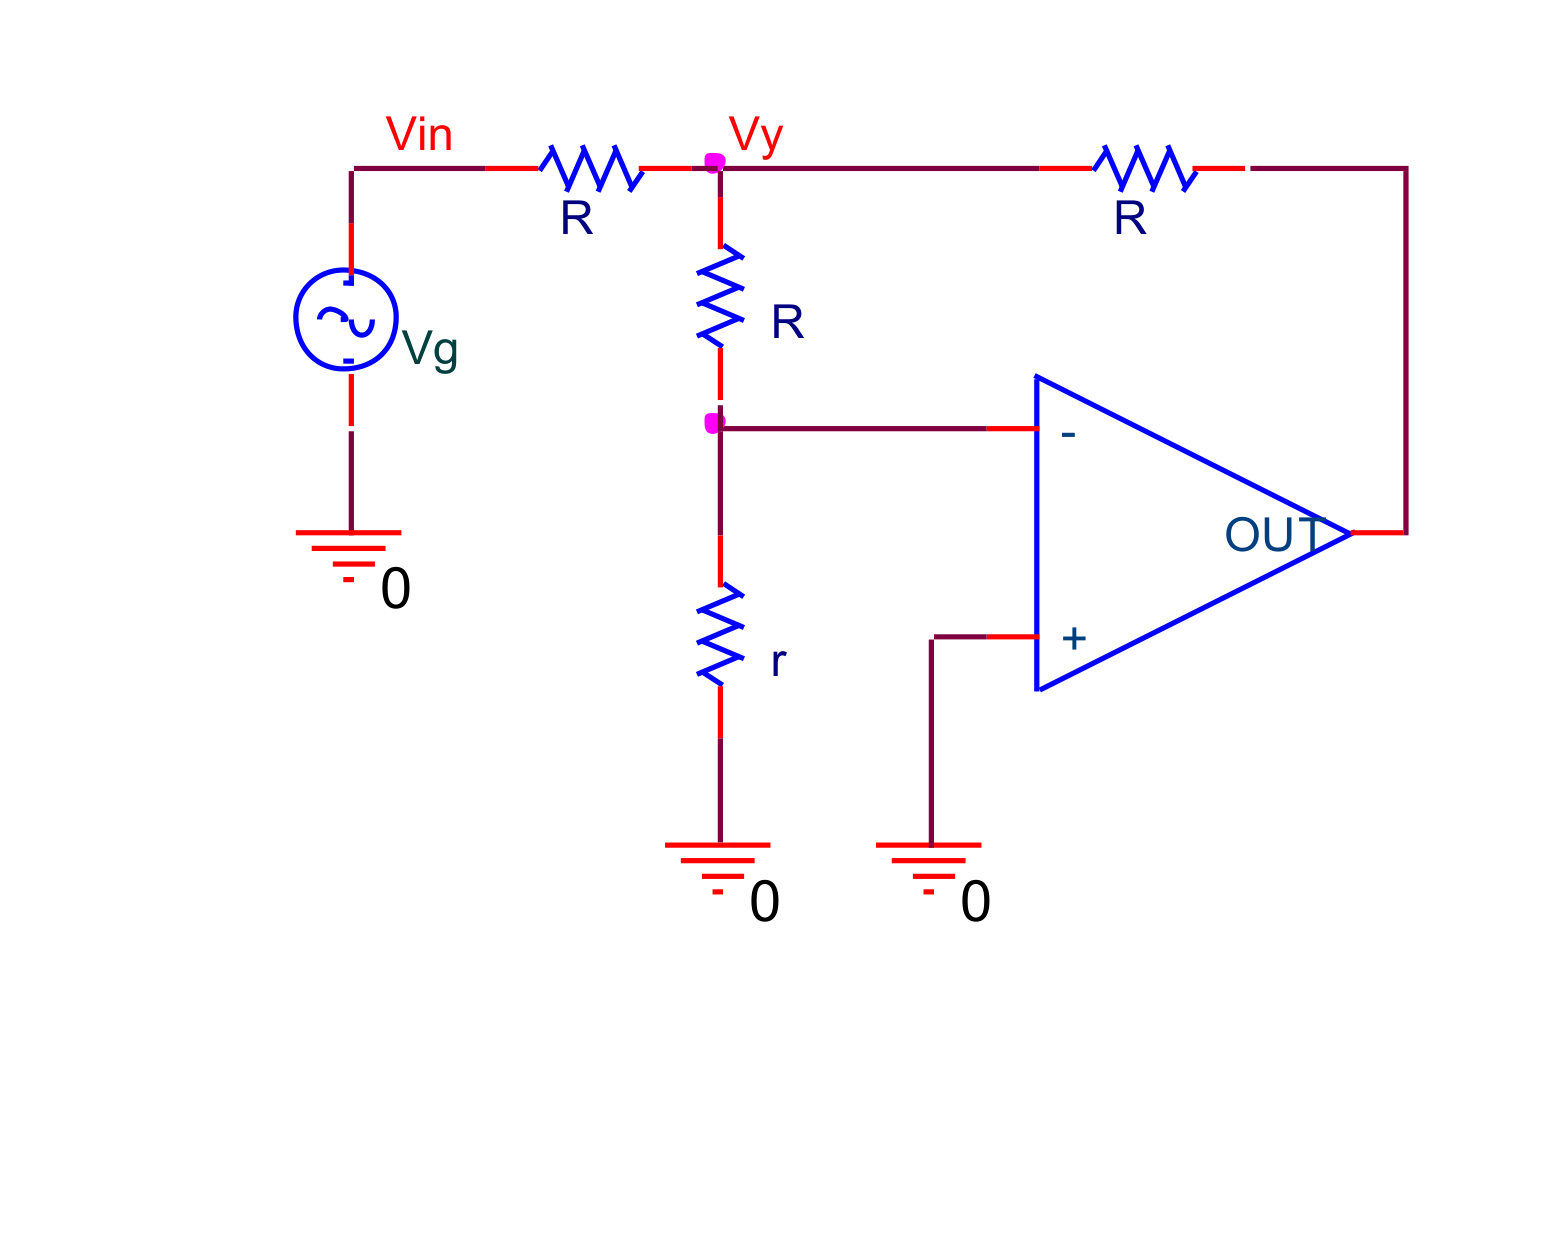
\includegraphics[keepaspectratio]{assets/figure9.png}}
\nopagebreak[4]

\begin{center}\textcolor{labteal}{\textit{Figure 8 - Figure 9: Circuit for open-loop gain measurement ($R\gg r$; $V_y$ is the node between the two $R$ resistors).}}\end{center}

For an \textbf{ideal} op-amp with virtual ground at \(V^- = V^+ = 0\):

Node \(V_y\) connects to \(V^-\) through \(r\); with virtual ground
\(V^- = 0\) and negligible current into the ideal input: \(V_y = 0\).

By KCL at \(V_y\):
\[\frac{V_g - V_y}{R} + \frac{V_o - V_y}{R} = \frac{V_y}{r} \;\Rightarrow\; V_g + V_o = 0\]

\[\boxed{\frac{V_y}{V_g} = 0, \quad \frac{V_o}{V_g} = -1}\]

\subsubsection{\texorpdfstring{8.2 Non-Ideal Case: Which Voltages to
Measure for
\(A_{OL}\)}{8.2 Non-Ideal Case: Which Voltages to Measure for A\_\{OL\}}}\label{non-ideal-case-which-voltages-to-measure-for-a_ol}

For a non-ideal op-amp with finite \(A_{OL}\):

\[V_y \approx \frac{V_g}{A_{OL}}\quad (\text{small but non-zero}),\quad V_o \approx -V_g\]

Measure \textbf{\(V_y\)} and \textbf{\(V_o\)}:

\[A_{OL} \approx \left|\frac{V_o}{V_y}\right|\]

This works because \(V_y \approx V^-\) (the op-amp's differential
input), and \(A_{OL} = V_o/(V^+ - V^-) = -V_o/V_y\) for \(V^+=0\).

\subsubsection{8.3 Required Input Signal}\label{required-input-signal}

\begin{itemize}
\tightlist
\item
  \textbf{Shape:} Sine wave (to measure RMS values unambiguously; square
  wave would introduce harmonics)
\item
  \textbf{Frequency:} Very low --- of order a few Hz
  (e.g.~\(1\text{–}10\,\mathrm{Hz}\)). The op-amp's open-loop bandwidth
  is only several Hz, so the flat (DC) value of \(A_{OL}\) is reached
  only \emph{below} this dominant pole; at \(100\,\mathrm{Hz}\) the
  open-loop gain is already rolling off. In the lab the measurement is
  therefore swept down to \(100\,\mathrm{Hz}\), \(10\,\mathrm{Hz}\) and
  \(1\,\mathrm{Hz}\) to trace the roll-off and extract the DC value.
\item
  \textbf{Amplitude:} \(V_g\) of order
  \(100\,\mathrm{mV}\)--\(1\,\mathrm{V_{RMS}}\), so that
  \(V_o = A_v\,V_g \approx V_g\) remains within \(\pm 15\,\mathrm{V}\)
  (not clipping), and \(V_y \approx V_g/A_{OL}\) is at the noise level
\end{itemize}

Expected signals: \(V_o \approx -V_g\) (large, clean sine);
\(V_y \approx V_g/A_{OL}\) (very small, of order \(\mu\mathrm{V}\),
noisy).

\subsubsection{\texorpdfstring{8.4 Scope Functions for Measuring the
Small Signal
\(V_y\)}{8.4 Scope Functions for Measuring the Small Signal V\_y}}\label{scope-functions-for-measuring-the-small-signal-v_y}

\begin{itemize}
\tightlist
\item
  \textbf{Averaging:} The scope averages \(N\) consecutive acquisitions;
  random noise decreases by \(\sqrt{N}\) while the coherent (periodic)
  \(V_y\) signal is preserved. Essential when \(V_y\) is at the noise
  floor.
\item
  \textbf{BW Limit:} Limits the oscilloscope's measurement bandwidth
  (e.g., to 20 kHz), cutting broadband noise that is irrelevant for a
  low-frequency measurement.
\item
  \textbf{Fine:} Allows fine adjustment of the vertical scale (e.g.,
  mV/div resolution), maximising the on-screen amplitude of \(V_y\) for
  more precise cursor measurements.
\end{itemize}

\newpage

\subsection{9. Op-Amp as an Integrator}\label{op-amp-as-an-integrator}

\subsubsection{9.1 Transfer Function (Figure
10)}\label{transfer-function-figure-10}

\pandocbounded{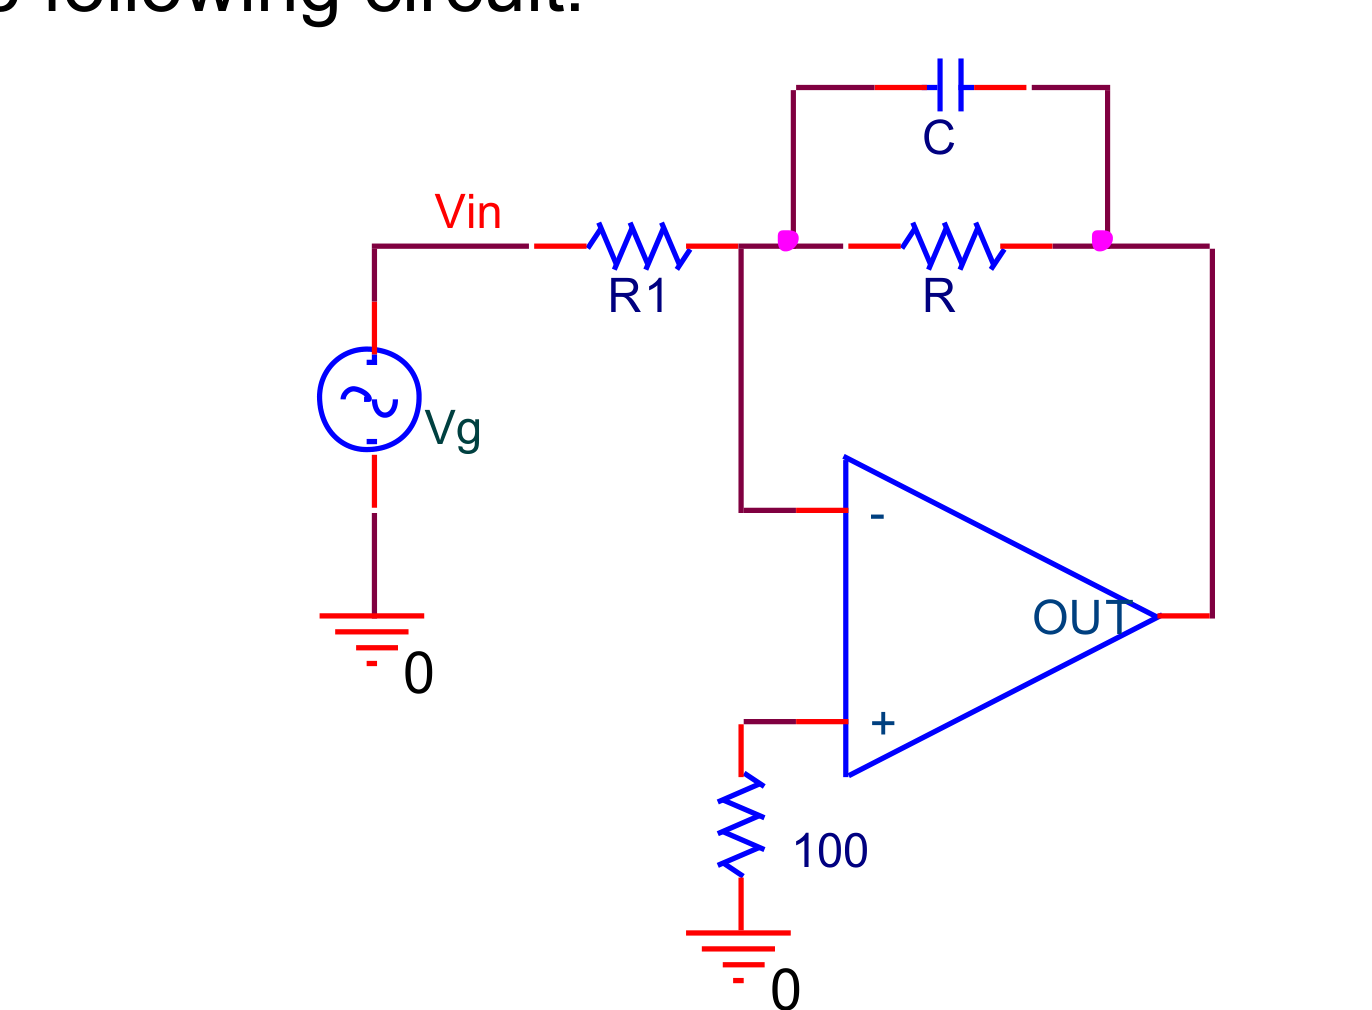
\includegraphics[keepaspectratio]{assets/figure10.png}}
\nopagebreak[4]

\begin{center}\textcolor{labteal}{\textit{Figure 9 - Figure 10: Integrator circuit with $R_1=10\,\mathrm{k}\Omega$, $R_f=20\,\mathrm{k}\Omega$ (parallel with $C=10\,\mathrm{nF}$) and $100\,\Omega$ on the $+$ input.}}\end{center}

The feedback impedance is \(Z_f = R_f \,\|\, \frac{1}{j\omega C}\):

\[H(j\omega) = -\frac{Z_f}{R_1} = -\frac{R_f}{R_1}\cdot\frac{1}{1+j\omega R_f C}\]

\subsubsection{9.2 Poles, Zeros, and Canonical
Form}\label{poles-zeros-and-canonical-form}

\[H(j\omega) = -\frac{R_f/R_1}{1 + j\omega/\omega_p}, \quad \omega_p = \frac{1}{R_f C}\]

\begin{itemize}
\tightlist
\item
  \textbf{1 pole}, \textbf{0 finite zeros}
\item
  Canonical form: \(H(jf) = \dfrac{-R_f/R_1}{1 + jf/f_p}\) with
  \(R_f/R_1 = 20\,\mathrm{k}/10\,\mathrm{k} = 2\),
  \(f_p\approx 796\,\mathrm{Hz}\)
\end{itemize}

\subsubsection{9.3 Dominant Pole}\label{dominant-pole}

\[f_p = \frac{1}{2\pi R_f C} = \frac{1}{2\pi\times 20\times10^3\times 10\times10^{-9}} \approx 796\,\mathrm{Hz}\]

\subsubsection{\texorpdfstring{9.4 Approximations for \(f \ll f_p\) and
\(f \gg f_p\)}{9.4 Approximations for f \textbackslash ll f\_p and f \textbackslash gg f\_p}}\label{approximations-for-f-ll-f_p-and-f-gg-f_p}

\[H_\text{low}(j\omega)\big|_{f\ll f_p} \approx -\frac{R_f}{R_1} = -2 \quad\text{(inverting amplifier)}\]

\[H_\text{high}(j\omega)\big|_{f\gg f_p} \approx -\frac{1}{j\omega R_1 C} \quad\text{(ideal integrator)}\]

\subsubsection{\texorpdfstring{9.5 Square-Wave Input at
\(f \ll f_p\)}{9.5 Square-Wave Input at f \textbackslash ll f\_p}}\label{square-wave-input-at-f-ll-f_p}

The circuit acts as an \textbf{inverting amplifier} (gain \(-2\)). The
output is a square wave, inverted and scaled by 2 relative to the input.

\subsubsection{\texorpdfstring{9.6 Square-Wave Input at
\(f \gg f_p\)}{9.6 Square-Wave Input at f \textbackslash gg f\_p}}\label{square-wave-input-at-f-gg-f_p}

The circuit acts as an \textbf{ideal integrator}. The integral of a
square wave is a \textbf{triangular wave}; the output is a triangular
wave 90° out of phase with the input, with amplitude inversely
proportional to frequency.

\subsubsection{\texorpdfstring{9.7 Simulation: Bode Plot and
\(f_p\)}{9.7 Simulation: Bode Plot and f\_p}}\label{simulation-bode-plot-and-f_p}

\begin{quote}
\textbf{{[}SIMULATION NEEDED --- 9.7{]}} Simulate the AC Bode plot of
Figure 10 in PSpice. From the flat low-frequency gain and the −3 dB
rolloff point, extract \(f_{-3\mathrm{dB}}\). Theoretical prediction:
\(f_p \approx 796\,\mathrm{Hz}\).
\end{quote}

\subsubsection{9.8 −3 dB Frequency from the
Simulation}\label{db-frequency-from-the-simulation}

Because the transfer function has a \textbf{single pole and no finite
zero}, the \(-3\,\mathrm{dB}\) frequency coincides with the dominant
pole:

\[f_{-3\mathrm{dB}} = f_p = \frac{1}{2\pi R_f C} \approx 796\,\mathrm{Hz}\]

The AC sweep therefore yields both quantities simultaneously: the
frequency where the gain has fallen by \(3\,\mathrm{dB}\)
(\(1/\sqrt{2}\) in magnitude) from its flat low-frequency value
\(|H|=R_f/R_1=2\) is the dominant pole \(f_p\).

\newpage

\subsection{10. Op-Amp as a Summation
Circuit}\label{op-amp-as-a-summation-circuit}

\subsubsection{10.1 Output of the Example Circuit (Figure
11)}\label{output-of-the-example-circuit-figure-11}

\pandocbounded{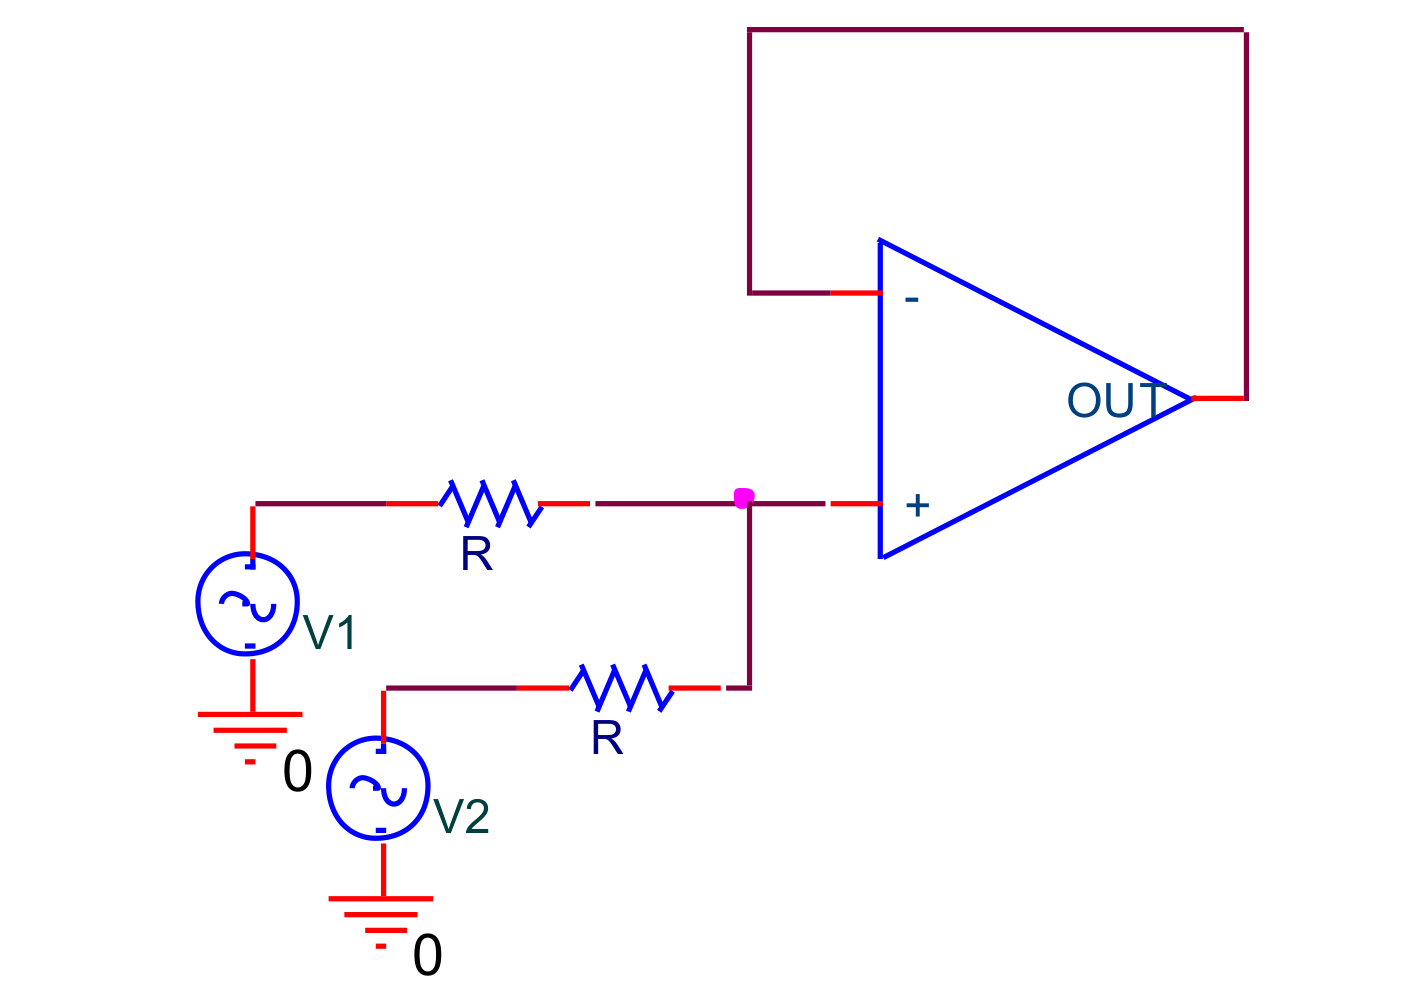
\includegraphics[keepaspectratio]{assets/figure11.png}}
\nopagebreak[4]

\begin{center}\textcolor{labteal}{\textit{Figure 10 - Figure 11: Inverting summing amplifier example ($R_1=R_2=R_f=R$).}}\end{center}

For the inverting summing amplifier with \(R_1 = R_2 = R_f = R\):

\[V_{out} = -\frac{R_f}{R_1}V_1 - \frac{R_f}{R_2}V_2 = -(V_1 + V_2)\]

\subsubsection{10.2 Mathematical
Operation}\label{mathematical-operation}

The circuit performs a \textbf{negated sum}: \(V_{out} = -(V_1 + V_2)\).
Up to a sign inversion, it adds the two inputs.

\subsubsection{\texorpdfstring{10.3 Calculation of \(F\) and
\(L\)}{10.3 Calculation of F and L}}\label{calculation-of-f-and-l}

\begin{itemize}
\tightlist
\item
  \(F\) = \textbf{first digit} of Shai Livshits' student ID:
  \(208632216 \Rightarrow F = 2\) (even)
\item
  \(L\) = \textbf{last digit} of Shai Livshits' student ID:
  \(208632216 \Rightarrow L = 6\) (even)
\end{itemize}

\subsubsection{10.4 Function Selection}\label{function-selection}

From the table, \textbf{F-even / L-even} assigns the function:

\[\boxed{V_{out} = -2V_1 + 2V_2}\]

\subsubsection{10.5 Circuit Design from the Master Circuit (Figure
12)}\label{circuit-design-from-the-master-circuit-figure-12}

The assigned function \(V_{out} = -2V_1 + 2V_2\) has a \(-2\)
coefficient on \(V_1\) (inverting) and a \(+2\) coefficient on \(V_2\)
(non-inverting), with \textbf{equal magnitudes}. This is exactly the
form produced by a \textbf{standard difference amplifier}, so there is
no need to brute-force the general master circuit --- by inspection the
topology is a one-op-amp difference amplifier with gain 2.

For a balanced difference amplifier with \(R_1\) from \(V_1\) to the
\((-)\) input, \(R_f\) in feedback, \(R_2\) from \(V_2\) to the \((+)\)
input, and \(R_3\) from \((+)\) to ground, with the matching condition
\(R_1=R_2\) and \(R_f=R_3\):

\[V_{out} = \frac{R_f}{R_1}\,(V_2 - V_1) = \frac{R_f}{R_1}\,V_2 - \frac{R_f}{R_1}\,V_1\]

Setting \(\dfrac{R_f}{R_1} = 2\) gives \(V_{out} = -2V_1 + 2V_2\), as
required. Choosing standard board values:

\[R_1 = R_2 = 10\,\mathrm{k}\Omega, \qquad R_f = R_3 = 20\,\mathrm{k}\Omega \quad (4\ \text{resistors total})\]

In terms of the master circuit (Figure 12): connect \(V_1\) through
\(10\,\mathrm{k}\Omega\) to the \((-)\) input, \(V_2\) through
\(10\,\mathrm{k}\Omega\) to the \((+)\) input, place a
\(20\,\mathrm{k}\Omega\) feedback resistor from output to \((-)\), tie
the \((+)\) input to ground through \(20\,\mathrm{k}\Omega\), and leave
any remaining free nodes/resistors disconnected. This satisfies the
``\(\leq 4\) resistors'' hint and uses only the matched-ratio symmetry
rather than the general solution.

\subsubsection{10.6 Simulation of the Designed
Circuit}\label{simulation-of-the-designed-circuit}

\begin{quote}
\textbf{{[}SIMULATION NEEDED --- 10.6{]}} Simulate the difference
amplifier above in PSpice with \(V_{g1}\) a square wave and \(V_{g2}\)
at \textbf{equal amplitude} to \(V_{g1}\). Attach: (i) \(V_g\) with
\(V_{in1}, V_{in2}\), (ii) both inputs \(V_{in1}, V_{in2}\) together
with the output \(V_{out}\). Annotate the prints with key amplitudes to
confirm \(V_{out} = -2V_{in1} + 2V_{in2}\)
(i.e.~\(V_{out}=2(V_{in2}-V_{in1})\)).
\end{quote}

\newpage

\subsection{11. 3 dB Frequency Measurement
(Self-Quiz)}\label{db-frequency-measurement-self-quiz}

\subsubsection{11.1 Horizontal Scale for 3 dB Frequency Measurement
(SWEEP
Mode)}\label{horizontal-scale-for-3-db-frequency-measurement-sweep-mode}

In SWEEP mode, the function generator sweeps from \(f_\text{start}\) to
\(f_\text{end}\) in \(T_\text{sweep}\) seconds. The horizontal scale
must be set so that the entire frequency range of interest (flat region
to well past the 3 dB frequency) fits within the 10-division screen.

A sweep time of \textbf{1 second} is standard. The horizontal scale is
then \(T_\text{sweep}/10 = \mathbf{100\,\mathrm{ms/div}}\).

\subsubsection{\texorpdfstring{11.2 Relationship Between \(V_{pp}\) at
Low Frequency and Amplitude at 3 dB
(LPF)}{11.2 Relationship Between V\_\{pp\} at Low Frequency and Amplitude at 3 dB (LPF)}}\label{relationship-between-v_pp-at-low-frequency-and-amplitude-at-3-db-lpf}

In the flat (low-frequency) region of an LPF, the output peak-to-peak
amplitude is \(V_{pp} = 2A_\text{flat}\).

At the \(-3\,\mathrm{dB}\) frequency, the amplitude drops by
\(1/\sqrt{2}\):

\[V_{-3\mathrm{dB}} = \frac{A_\text{flat}}{\sqrt{2}} = \frac{V_{pp}}{2\sqrt{2}} = \frac{V_{pp}}{\sqrt{2}\cdot 2} \approx 0.354\, V_{pp}\]

Equivalently, \(V_{pp}\) at 3 dB equals \(V_{pp,\text{flat}}/\sqrt{2}\).

\subsubsection{11.3 Measuring the 3 dB Frequency of an
HPF}\label{measuring-the-3-db-frequency-of-an-hpf}

\begin{enumerate}
\def\labelenumi{\arabic{enumi}.}
\tightlist
\item
  \textbf{Perform an AC sweep.} Confirm the response resembles an HPF
  (low amplitude at low \(f\), flat at high \(f\)).
\item
  \textbf{Identify the flat high-frequency region.} Measure
  \(V_{out,\text{RMS}}\) and \(V_{in,\text{RMS}}\) at a frequency where
  the gain is flat; compute \(A_\text{flat} = V_{out}/V_{in}\).
\item
  \textbf{Compute the −3 dB level:}
  \(A_{-3\mathrm{dB}} = A_\text{flat}/\sqrt{2}\).
\item
  \textbf{Decrease frequency from the flat region} while continuously
  monitoring \(V_{out,\text{RMS}}/V_{in,\text{RMS}}\). Keep the signal
  on screen (several cycles, good resolution).
\item
  When the ratio falls to \(A_{-3\mathrm{dB}}\), record the frequency
  --- this is \(f_{-3\mathrm{dB}}\).
\item
  \textbf{Caution:} at very low frequencies, one period may exceed the
  scope's useful time window; ensure at least 5 full cycles are visible.
  Do not go below about \(10\,\mathrm{Hz}\) unless the expected 3 dB
  frequency is there. Also verify the output is a clean sinusoid (not
  distorted) before recording.
\end{enumerate}

\newpage

\subsection{12. Table Measurement --- Frequency Dependence
(Self-Quiz)}\label{table-measurement-frequency-dependence-self-quiz}

When filling the quantitative measurement tables in the lab, keep the
following rules:

\begin{itemize}
\tightlist
\item
  \textbf{Always measure the input as well}, since it does not
  necessarily stay constant across frequency; gain is the ratio of the
  \emph{transfer-function} output to input (not always the circuit's
  terminals).
\item
  \textbf{Prefer RMS over \(V_{pp}\)}: electrical noise can create
  spurious peaks that corrupt a \(V_{pp}\) reading, whereas RMS averages
  them out.
\item
  \textbf{Sign convention:} if a V/V (gain) column is requested, include
  the sign when it is definitive (e.g.~negative for an inverting stage).
  If a dB column is requested instead, compute
  \(A_\mathrm{dB} = 20\log_{10}|A|\).
\item
  \textbf{Phase:} when measuring phase, take the phase of \(V_o/V_i\)
  (not \(V_i/V_o\)) and add \(180^\circ\) whenever the sign flips.
\item
  \textbf{Linearity:} the transfer-function concept assumes a linear
  system, so both input and output must be \textbf{undistorted sine
  waves}. If the output is distorted, reduce the input amplitude until
  the circuit operates linearly before recording.
\end{itemize}

\subsection{References}\label{references}

\begin{itemize}
\tightlist
\item
  Sedra, A. S., \& Smith, K. C. \emph{Microelectronic Circuits}, 6th
  ed.~Oxford University Press. Chapters 2, 12.
\item
  Millman, J., \& Halkias, C. \emph{Integrated Electronics}. Chapters
  15--16.
\item
  TL071M, TL061M, LM741 Datasheets (Texas Instruments / National
  Semiconductor).
\item
  ``How to read an op-amp data sheet'' --- course Moodle resource.
\end{itemize}

\end{document}
